\documentclass[UTF8,fontset=fandol,11pt,a4paper]{ctexart}
\usepackage[paperwidth=200mm,paperheight=267mm,left=20mm,right=20mm,top=21mm,bottom=19mm,headheight=16pt]{geometry}
\usepackage{amsmath,amssymb,booktabs,tabularx,graphicx,xcolor,hyperref,fancyhdr,indentfirst,listings}
\usepackage{tikz}
\definecolor{wine}{HTML}{833A42}
\definecolor{ink}{HTML}{22292C}
\definecolor{quiet}{HTML}{565E64}
\definecolor{shade}{HTML}{F5F2EF}
\hypersetup{colorlinks=true,urlcolor=wine,linkcolor=wine,filecolor=wine,pdftitle={Redflag 实时光照与采样}}
\setlength{\parindent}{2\ccwd}
\setlength{\parskip}{5pt plus 1pt}
\linespread{1.1}
\ctexset{section={format=\Large\bfseries\color{wine},afterindent=true},subsection={format=\large\bfseries\color{ink},beforeskip=8pt,afterskip=2pt,afterindent=true}}
\setcounter{secnumdepth}{1}
\setcounter{tocdepth}{1}
\pagestyle{fancy}\fancyhf{}\fancyhead[L]{\small Redflag\enspace / \enspace 实时光照与采样}
\fancyhead[R]{\small\color{quiet}\nouppercase{\leftmark}}\fancyfoot[R]{\thepage}
\renewcommand{\sectionmark}[1]{\markboth{#1}{}}
\renewcommand{\headrulewidth}{.35pt}
\setlength{\emergencystretch}{2em}
\lstset{basicstyle=\ttfamily\small,backgroundcolor=\color{shade},frame=l,rulecolor=\color{wine},xleftmargin=4mm,framexleftmargin=2mm,columns=fullflexible,keepspaces=true,showstringspaces=false,breaklines=true}
\newcommand{\term}[1]{{\small\color{quiet}(#1)}}
\newcommand{\pair}[5][.48\linewidth]{\begin{center}\begin{minipage}{#1}\centering\includegraphics[width=\linewidth]{../../../output/#2}\\[-2pt]{\small #3}\end{minipage}\hfill\begin{minipage}{#1}\centering\includegraphics[width=\linewidth]{../../../output/#4}\\[-2pt]{\small #5}\end{minipage}\end{center}}
\newenvironment{fields}{\par\noindent\tabularx{\linewidth}{@{}p{.30\linewidth}X@{}}\toprule 字段或入口 & 读写时的含义\\\midrule}{\bottomrule\endtabularx}
\begin{document}
\section*{实时光照与采样}
\markboth{阅读与复现}{}
走廊里两盏灯同时照到地板，给同一点的两份亮度相加就得到直接光。灯多时，也可以抽查其中一盏，再用选中它的概率估计总和。后面介绍的 ReSTIR 还会用上相邻像素与上一帧挑出来的灯。

本册的比较图来自 Redflag。Sponza 定量测试把模型缩到最大跨度 20 个世界单位，各种采样方法都看同一条走廊。为了单独观察噪声，这组基准采用贴图的平均底色和纯漫反射。编辑器中的挂毯则保留花纹。Vulkan 先画出相机看见的三角形和带花纹的底色，计算着色器再沿光线去找灯前的遮挡物，以及下一次反射碰到的表面。
\pair[.40\linewidth]{profiling/gi/direct-reference.png}{逐灯求和得到的直接光}{profiling/gi/indirect-reference.png}{墙面反射一次后的间接光}
{\small\linespread{.94}\selectfont\setlength{\parskip}{0pt}\tableofcontents}
\clearpage
\section{显卡上的数组、图像和上一帧}
在 GAMES104 的引擎分层里，上层知道要算什么，底层知道怎么把工作交给某一种图形接口。Redflag 中的 \texttt{Scene} 保存模型和点光源，\texttt{GlobalIllumination} 决定对哪些表面追踪光线，\texttt{ScreenEffects} 决定要运行哪个屏幕效果。这两者只向 \texttt{ComputeDevice} 提交程序、资源和工作组数。实际分配 Vulkan 内存、把资源交给着色器并提交命令的是 \texttt{VulkanComputeDevice}。游戏脚本平时操作的是场景实体，只有编写新的 GPU 效果才需要碰这些接口。

\subsection{从一个像素读懂三帧}
以 $7\times5$ 的测试图为例。CPU 先准备 35 个整数 $0,\ldots,34$，另分配两张每像素四个浮点数的图。第一张清零，第二张留作第一次的输出。每一帧的着色器读上一张图、更新对应整数，把新值写入另一张图。要保留历史只须交换两张图的角色，数据仍留在显卡可以访问的资源里。

\noindent{\small\color{quiet}C++ 接口调用示例\quad\href{run:../../tests/ComputeTests.cpp}{\texttt{ComputeTests.cpp}}}\par\nopagebreak
\begin{lstlisting}[escapeinside={(*@}{@*)}]
auto numbers = device.CreateBuffer(sizeof(initial), initial);
auto first   = device.CreateImage(7, 5, zeros);
auto second  = device.CreateImage(7, 5);
auto program = device.CreatePipeline(code, bytes,
    {Buffer, Image, Image}, sizeof(uint32_t));
(*@{\footnotesize\color{quiet}两个方向各派两组线程；本帧读第一张图，写第二张图。}@*)
device.Dispatch(program, {numbers, first, second}, &frame, 2, 2);
\end{lstlisting}
这里省略了枚举类型名前缀。每组覆盖 $4\times4$ 个像素，宽 7、高 5，两个方向都向上取整得到两组。超出图像的线程直接返回。数组和图的排列必须与着色器中的声明相同；最后的 \texttt{frame} 指向当前帧号，只有四字节。前三帧的输出依次是第二、第一、第二张图。测试读回所有整数及像素分量，第三帧最后一像素红色通道应等于 112。

\subsection{提交与读取}
Khronos 的计算着色器教程从工作组和读写依赖入手。Redflag 在 CPU 端调用 \texttt{Dispatch} 时先记录资源和计算工作，再提交队列。当前版本等该次提交完成后才返回，下一次计算可以安全读取结果。连续处理多道效果时，这个约定简化了排错，也会让 CPU 等待多次。评估异步提交应先把 GPU 时间查询与 CPU 等待分开记录，再比较同一场景的帧耗时。

\texttt{Readback} 将指定资源的字节读进 CPU 提供的数组，适合测试逐值核验。编辑器显示画面可以直接读取显卡输出，经显示着色器写进 ImGui 的纹理，从而省掉逐帧回读。

在项目的 \texttt{tests} 目录执行 \texttt{run\_compute\_tests.cmd}，就能单独验证这三帧。CPU 端的读回检查写在 \texttt{ComputeTests.cpp}，对应的计算着色器名为 \texttt{ComputeHistory.comp}。

{\small 参考\quad\href{https://docs.vulkan.org/tutorial/latest/11_Compute_Shader.html}{Khronos 的计算着色器}\quad
\href{https://games104.boomingtech.com/sc/course-list/}{GAMES104，第 2 讲}\quad
\href{https://github.com/TheCherno/Hazel/blob/master/Hazel/src/Hazel/Renderer/Texture.h}{Hazel 的资源接口}\quad
\href{https://gameenginebook.com/}{Gregory，《游戏引擎架构》}}

\clearpage
\section{方向光与投影}

两张图里的兔子、地面和相机都在原处。场景只留一盏方向光，阳光从兔子的左上方照来。看右图，耳朵上沿受光，腹部下面的地面落在阴影里。旧版里连耳朵也看不见。用 RenderDoc 查看时，底色和深度中都有模型，最后送给面板的光照却全是零。顺着这条线索回到编辑器，才发现它交给 Vulkan 的灯光列表只收集了点光源。

\pair{validation/directional-light/bunny-before.png}{旧版，光照图全黑}{validation/directional-light/bunny-after.png}{修复后，太阳照亮兔子与地面}
{\small\color{quiet}Redflag 正式 Vulkan 编辑器的场景面板。Stanford Bunny，$384\times246$，RenderDoc 第 24 帧。两次均关闭间接光和环境光，保留相同的 TAA 和曝光。}

把台灯从一米外挪到两米外，原来落在一小块墙上的光就分散到更大的面积上。太阳离这间屋子足够远，从地面走到兔子身边，收到的阳光可以看成来自同一方向，强度也相同。描述这盏灯只需它的方向、颜色和强度。移动灯的实体不会移动阴影，转动灯才会改变阴影的朝向。\href{https://pbr-book.org/4ed/Light_Sources/Distant_Lights}{PBRT 第四版 §12.3}

设地板的粗糙表面向各个方向均匀反光，能反射的比例是 $\rho$。用单位向量 $\mathbf n$ 表示地板的朝向，$\mathbf l$ 从地板指向光源。太阳正对地板时，这块面积能接住整束光；转过 $60^\circ$，它从太阳方向看去只剩一半宽，收到的光也减半。这个比例就是 $\mathbf n\cdot\mathbf l=\cos\theta$。再从地面向太阳检查一次遮挡，有模型挡住时取 $V=0$，一路通畅时取 $V=1$。若 $E$ 表示正对太阳时收到的光，漫反射送向相机的亮度为
\[
 L_o=\frac{\rho}{\pi}\,E\,\max(0,\mathbf n\cdot\mathbf l)\,V .
\]
这里除以 $\pi$，使表面向上方所有方向反射的光加起来等于它收到的光乘 $\rho$。Redflag 的直接光还会计算材质高光。算探针时，光线先找到墙面，再用上式估计墙向房间反射的光。

{\small GLSL，摘自 \path{Renderer/GI/Shaders/LightSource.glsl} 的 \texttt{sampleLight}（方向光分支）。}
\begin{lstlisting}
toLight = source.xyz;             // CPU 已把方向换成从表面指向太阳
distanceToLight = 3.402823466e38; // 查遍场景中沿这条射线的遮挡物
return 1.;                       // 光照强度在场景各处相同
\end{lstlisting}
场景组件保存的是光线传播的方向，从表面往回找太阳时要反向。上面的距离取浮点数能表示的最大有限值，只供查找遮挡物使用。画雾时，视点到墙面之间实际有多长一段雾，就对那段距离计算透射。近墙和远墙可以受到一样强的日照，远墙前的空气却能把更多光散射进镜头。\href{run:../validation/directional/DirectionalLight_capture.rdc}{两面墙的 RenderDoc 实测帧}

\expandafter\def\csname metric-width\endcsname{161}
\expandafter\def\csname metric-height\endcsname{91}
\expandafter\def\csname metric-vertical_fov_degrees\endcsname{65}
\expandafter\def\csname metric-display_exposure\endcsname{4}
\expandafter\def\csname metric-visible_pixels\endcsname{14501}
\expandafter\def\csname metric-lights_for_cluster_test\endcsname{49}
\expandafter\def\csname metric-ao_min\endcsname{0.023615}
\expandafter\def\csname metric-ao_mean\endcsname{0.89868}
\expandafter\def\csname metric-ao_negligible_radius_mean\endcsname{0.99974}
\expandafter\def\csname metric-ssr_hit_fraction\endcsname{0.36335}
\expandafter\def\csname metric-ssr_repeat_max_difference\endcsname{0}
\expandafter\def\csname metric-ssr_roughness_image_mse\endcsname{0.00017208}
\expandafter\def\csname metric-taa_first_rgb_mse\endcsname{0}
\expandafter\def\csname metric-taa_reset_max_weight\endcsname{0}
\expandafter\def\csname metric-taa_frame8_mean_weight\endcsname{0.875}
\expandafter\def\csname metric-taa_moved_frame_reused_fraction\endcsname{0.41042}
\expandafter\def\csname metric-single_frame_vs_eight_jitters_mse\endcsname{0.0016975}
\expandafter\def\csname metric-taa_vs_eight_jitters_mse\endcsname{1.1057e-16}
\expandafter\def\csname metric-cluster_max_absolute_rgb_error\endcsname{1.4901e-07}
\expandafter\def\csname metric-cluster_mean_candidates\endcsname{18.109}
\expandafter\def\csname metric-cluster_zero_lights_rgb_max\endcsname{0}
\expandafter\def\csname metric-mirror-stripe-ratio\endcsname{0.212}
\expandafter\def\csname metric-mirror-white-r\endcsname{3.721}
\expandafter\def\csname metric-mirror-white-g\endcsname{0.516}
\expandafter\def\csname metric-mirror-gray-r\endcsname{0.842}
\expandafter\def\csname metric-mirror-gray-g\endcsname{0.145}
\expandafter\def\csname metric-mirror-black-r\endcsname{0.066}
\expandafter\def\csname metric-mirror-black-g\endcsname{0.059}
\expandafter\def\csname metric-mirror-board-r\endcsname{0.008}
\expandafter\def\csname metric-mirror-board-g\endcsname{0.069}
\expandafter\def\csname metric-rough-reference-mean_rgb_mse\endcsname{0}
\expandafter\def\csname metric-rough-reference-adjacent_rgb_mse\endcsname{0}
\expandafter\def\csname metric-rough-reference-bright_minus_middle_red\endcsname{0.47532}
\expandafter\def\csname metric-rough-raw-mean_rgb_mse\endcsname{0.58163}
\expandafter\def\csname metric-rough-raw-adjacent_rgb_mse\endcsname{1.1603}
\expandafter\def\csname metric-rough-raw-bright_minus_middle_red\endcsname{0.56071}
\expandafter\def\csname metric-rough-filtered-mean_rgb_mse\endcsname{0.059193}
\expandafter\def\csname metric-rough-filtered-adjacent_rgb_mse\endcsname{0.11625}
\expandafter\def\csname metric-rough-filtered-bright_minus_middle_red\endcsname{0.55329}
\expandafter\def\csname metric-reference-mean\endcsname{0.011098}
\expandafter\def\csname metric-direct-1spp-mse\endcsname{0.16609}
\expandafter\def\csname metric-direct-1spp-mean_rgb\endcsname{0.10873}
\expandafter\def\csname metric-direct-1spp-reused_fraction_visible\endcsname{0}
\expandafter\def\csname metric-direct-1spp-reused_fraction_positive\endcsname{0}
\expandafter\def\csname metric-direct-8spp-mse\endcsname{0.021521}
\expandafter\def\csname metric-direct-8spp-mean_rgb\endcsname{0.11019}
\expandafter\def\csname metric-direct-8spp-reused_fraction_visible\endcsname{0}
\expandafter\def\csname metric-direct-8spp-reused_fraction_positive\endcsname{0}
\expandafter\def\csname metric-restir-di-mse\endcsname{0.011318}
\expandafter\def\csname metric-restir-di-mean_rgb\endcsname{0.11226}
\expandafter\def\csname metric-restir-di-reused_fraction_visible\endcsname{90.993}
\expandafter\def\csname metric-restir-di-reused_fraction_positive\endcsname{94.681}
\expandafter\def\csname metric-indirect-1spp-mse\endcsname{0.022379}
\expandafter\def\csname metric-indirect-1spp-mean_rgb\endcsname{0.011477}
\expandafter\def\csname metric-indirect-1spp-reused_fraction_visible\endcsname{0}
\expandafter\def\csname metric-indirect-1spp-reused_fraction_positive\endcsname{0}
\expandafter\def\csname metric-indirect-8spp-mse\endcsname{0.0018102}
\expandafter\def\csname metric-indirect-8spp-mean_rgb\endcsname{0.011152}
\expandafter\def\csname metric-indirect-8spp-reused_fraction_visible\endcsname{0}
\expandafter\def\csname metric-indirect-8spp-reused_fraction_positive\endcsname{0}
\expandafter\def\csname metric-ddgi-mse\endcsname{4.1025e-05}
\expandafter\def\csname metric-ddgi-mean_rgb\endcsname{0.0090435}
\expandafter\def\csname metric-ddgi-reused_fraction_visible\endcsname{0}
\expandafter\def\csname metric-ddgi-reused_fraction_positive\endcsname{0}
\expandafter\def\csname metric-restir-gi-mse\endcsname{0.0003678}
\expandafter\def\csname metric-restir-gi-mean_rgb\endcsname{0.01017}
\expandafter\def\csname metric-restir-gi-reused_fraction_visible\endcsname{91.597}
\expandafter\def\csname metric-restir-gi-reused_fraction_positive\endcsname{93.619}
\newcommand{\measured}[1]{\csname metric-#1\endcsname}
\clearpage
\section{从两盏灯到一个采样估计}
\label{lesson-sampling}
% 前置知识
地板上一点同时看得到两盏灯。为了便于心算，假设它们给这一点带来的亮度分别是 2 和 6，真实总和就是 8。每次只肯花一条阴影光线时，程序只能检查其中一盏。它需要保存“我是以多大的机会选到这盏灯的”，才能用这一次观察估计两盏灯的总和。PBRT 第四版第 2 章从同样的期望定义出发；到 ReSTIR 章节时，被挑选的对象会从灯变成整条反射路径。

% 公式推导
两盏灯各有一半机会被选中。直接返回 2 或 6，多次试验的平均值会靠近 4，因为只看到了一半的灯。分别除以选中它的概率，返回值变成 4 或 12，平均值就靠近 8。期望是按每个结果发生的概率加权得到的平均。估计量的期望恰好等于目标时，称它无偏。一次采样究竟偏离 8 多远，则要看方差。这里方差是 $(4-8)^2/2+(12-8)^2/2=16$。若事先知道亮度之比，用 $1/4,3/4$ 的概率选两盏灯，两种结果都返回 8。这就是重要性采样的出发点。在有遮挡的真实场景中，真实亮度恰好是我们还没算出来的量，只能用便宜的近似来选灯。

% 公式
对于离散灯号 $i$，记贡献为 $f_i$，选灯概率为 $p_i$。对于连续方向 $\omega$，概率密度 $p(\omega)$ 表示单位立体角内分配多少概率；一个小区域的概率近似为密度乘上该区域的立体角。
\[
\widehat L=f_i/p_i,\qquad
\mathbb E[\widehat L]=\sum_i p_i f_i/p_i=\sum_i f_i,\qquad
\widehat I_N=\frac1N\sum_{k=1}^N\frac{f(\omega_k)}{p(\omega_k)}.
\]
任何有贡献的候选都须有机会被选中。独立样本取平均会让方差除以 $N$；重复用同一条旧路径时，样本间产生相关性，这条方差结论就不能直接套用。

\begin{center}\begin{tikzpicture}[x=.95cm,y=.9cm]
\draw[rounded corners,gray!50,fill=shade] (-.45,-1.05) rectangle (12.45,1.35);
\fill[wine!28] (0,0) rectangle (3,.7);
\fill[teal!22] (3,0) rectangle (12,.7);
\draw[gray] (0,0) rectangle (12,.7);\draw[gray] (3,0)--(3,.7);
\node at (1.5,.35){灯 A};\node at (7.5,.35){灯 B};
\node[above] at (1.5,.7){25\%};\node[above] at (7.5,.7){75\%};
\draw[->,thick] (1.2,-.46)--(1.2,-.02);\draw[->,thick] (7.44,-.46)--(7.44,-.02);
\node[below] at (1.2,-.42){$u=0.10$};\node[below] at (7.44,-.42){$u=0.62$};
\end{tikzpicture}\\{\small 本册绘制。一个随机数只落入一段，段越长，对应灯被抽到的机会越大。}\end{center}

\clearpage
% 逐行伪代码
\subsection{只追踪一盏灯}
一张累积概率表 \term{CDF} 把 $[0,1)$ 划成不同长度的区间。掷出 $0.10$ 落入第一段，掷出 $0.62$ 落入第二段。PBRT 的逆变换采样把这个办法推广到连续分布。
\noindent{\small\color{quiet}教学伪代码，手算例\quad\href{run:../../Redflag/src/Redflag/Renderer/GI/Shaders/GI.comp}{\texttt{GI.comp}}}\par\nopagebreak
\begin{lstlisting}[escapeinside={(*@}{@*)}]
probability = [0.25, 0.75]
endOfRange  = [0.25, 1.00]
u = uniformRandom(0, 1)
i = firstIndexWhere(endOfRange > u)
(*@{\footnotesize\color{quiet}一盏灯只在部分帧被抽到，除以选中概率补回其份额。}@*)
return contribution(i) / probability[i]
\end{lstlisting}

% 接口与数据结构
\begin{fields}
\texttt{GILight} & 世界位置决定方向和距离，RGB 强度决定三个颜色通道各自的光量。\\
\texttt{candidate} & 直接光分支均匀挑一盏灯，临时权重为灯数；间接光分支在表面上方挑一个方向。\\
\texttt{SetSeed} & 固定一串随机数的起点，重复绘制时便于逐像素检查。换种子后可观察误差的波动。\\
\end{fields}

% 验证标准
拿纸列出前面的两个结果，分别算 $\mathbb E[\widehat L]$ 和 $\mathbb E[(\widehat L-8)^2]$。再打开项目的 Sponza 基准。它将 16 盏点光源逐盏求和作为直接光参考，误差在曝光前的线性 RGB 上计算。把屏幕 PNG 再相减会把显示曲线也算进误差。后面的章节沿用这个区别。

\par\noindent{\small\color{quiet}材料索引\enspace \href{https://pbr-book.org/4ed/Monte_Carlo_Integration/Monte_Carlo_Basics}{PBRT 第四版 §2.1}\enspace · \enspace \href{https://pbr-book.org/4ed/Monte_Carlo_Integration/Sampling_Using_the_Inversion_Method}{§2.3 逆变换采样}\enspace · \enspace \href{https://github.com/mmp/pbrt-v4}{PBRT 源码}\enspace · \enspace \href{https://sites.cs.ucsb.edu/~lingqi/teaching/games101.html}{GAMES101 课程}\enspace · \enspace \href{run:../../docs/latex/lighting/sampling.tex}{可编辑笔记}}
\clearpage
\section{点光源下的金属高光}

把一块橙色面板放在三盏灯下，保持底色、相机和灯的位置不动。中图和右图都是金属，右图的表面更光滑。沿面板上半部寻找最亮的一点，粗糙表面把光反射到较宽的一片方向，光滑表面把它集中到较窄的一束。灯罩、金属把手和漆面会因此显出不同的质感。

\begin{center}
\begin{tabular}{@{}ccc@{}}
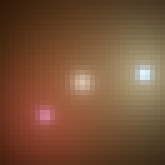
\includegraphics[width=.22\linewidth]{../../../output/profiling/point-materials/dielectric.png}&

\includegraphics[width=.22\linewidth]{../../../output/profiling/point-materials/rough-metal.png}&
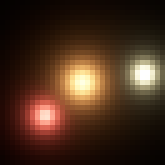
\includegraphics[width=.22\linewidth]{../../../output/profiling/point-materials/smooth-metal.png}\\
{\small 非金属，粗糙度 0.25}&{\small 金属，粗糙度 0.70}&{\small 金属，粗糙度 0.25}
\end{tabular}
\end{center}

这组三灯实测在 Vulkan 画出 $33\times33$ 个像素，三幅图使用相同曝光。正中像素的线性红通道依次为 1.170、0.346、16.105。最后一个数超过 1，着色器仍要保留它，显示时才压到屏幕能表现的亮度。若只拿底色乘光强，这三张图就无法区分。

设从面板指向灯、眼睛的单位向量分别为 $l,v$，表面法线为 $n$。能把这盏灯直接反进眼睛的小镜面朝向 $h=(l+v)/\lVert l+v\rVert$。GGX 用 $D$ 描述多少小镜面朝向 $h$，用 $G$ 描述其中有多少能同时看见灯和眼睛。粗糙度 $r$ 决定 $D$ 的宽度。代码取 $\alpha=\max(r^2,0.002)$，让最光滑的材质仍有一个有限宽度的高光；0.002 是项目的数值下限。$F$ 是光在这次反射中留下的比例，会随角度改变。光垂直照在普通非金属上时，glTF 取 $F_0=0.04$；金属则用自己的底色作 $F_0$。镜面反射函数为
\[
 f_s=\frac{D(h)\,G(l,v)\,F(v,h)}{4(n\cdot l)(n\cdot v)}.
\]
当前点落在灯的正面、且能看见灯时，把镜面与漫反射两项相加，再乘 $n\cdot l$ 和到达此点的灯光。点光源的强度随距离平方衰减，接近组件设定的半径时平滑降到零。分簇绘制先剔除照不到这里的灯，对留下的灯仍查相同的阴影、使用同一反射公式。

glTF 粗糙度贴图的绿色通道保存粗糙度，蓝色保存金属度。比如绿色的字节值为 64，粗糙度因子为 0.8，着色时取 $0.8\times64/255=0.201$。这两个通道都直接除以 255，底色贴图才需要从 sRGB 解码。DDGI 只传播漫反射，用 $(1-m)c$ 表示金属度 $m$、底色 $c$ 的漫反射率。在两面墙的测试里，经过两墙到达相机的红光为 0.277；将反光墙或接收墙分别换成纯金属，这项都降为零。

{\small\href{https://registry.khronos.org/glTF/specs/2.0/glTF-2.0.html\#appendix-b-brdf-implementation}{glTF 2.0 附录 B}\quad
\href{https://pbr-book.org/4ed/Reflection_Models/Roughness_Using_Microfacet_Theory}{PBRT 第四版 §9.6}\quad
\href{run:../../Redflag/src/Redflag/Renderer/GI/Shaders/PointLighting.glsl}{点光源着色源码}\quad
\href{run:../profiling/point-materials/README.md}{原图、实测与操作方法}}

\clearpage
\section{探针怎样估计间接光}
\label{lesson-ddgi}
% 前置知识
看左图里兔子的下巴和尾巴。点光源照不到的一侧几乎融进黑色背景。地面也受到了照明，其中一部分光从地面反射回来，能照到兔子的背光面。把单独算出的这部分光（中图）加到左图上，右图里就能辨出尾巴的轮廓。

\begin{center}
\begin{tabularx}{\linewidth}{@{}XXX@{}}
\centering\arraybackslash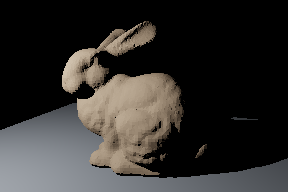
\includegraphics[width=\linewidth]{figures/bunny-direct.png} &
\centering\arraybackslash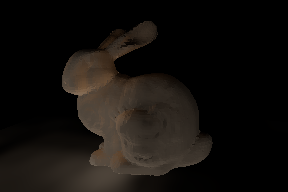
\includegraphics[width=\linewidth]{figures/bunny-bounce.png} &
\centering\arraybackslash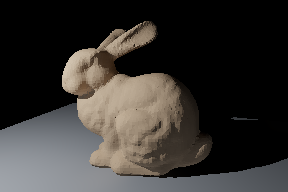
\includegraphics[width=\linewidth]{figures/bunny-combined.png}\\[-1pt]
\centering\arraybackslash\small 直接光 &
\centering\arraybackslash\small DDGI 间接光 &
\centering\arraybackslash\small 两者相加
\end{tabularx}\\[2pt]
{\footnotesize\color{quiet}Stanford Bunny，Redflag Vulkan，$288\times192$。探针计算一次漫反射，连续更新 8 帧；三张图使用同一曝光。}
\end{center}

要估算各处能收到多少反射光，可以在场景中布置一组探针，让它们从各自的位置向四周取样。给兔子着色时，就从附近的探针读取间接光。移到 Sponza 的走廊，还要当心墙另一侧的探针。探针会记下光线走多远碰到了表面，查询时这份记录能帮助判断两者之间是否隔着墙。

% 公式推导
GAMES101 的余弦项可以用一束平行光照在斜纸上的覆盖面积来理解。把单位方向 $\omega$ 与单位法线 $n$ 做点积，得到 $\cos\theta$。对墙面上半球的来光按这个值加权，就是辐照度 $E$。在 PBRT 的漫反射模型中，反射率为 $\rho$ 的墙把这些光转换为出射辐亮度 $L_o=\rho E/\pi$。现在把取样方向的密度选成 $\cos\theta/\pi$，代入采样估计式，余弦和 $\pi$ 正好抵消。此处 $\rho$ 对应 $(1-m)c$，一块纯金属板的 $m=1$，不把它的底色加进漫反射。探针累加追踪得到的来光，平均值直接估计 $E/\pi$。

% 公式
\[
 E(n)=\int_{\Omega^+}L_i(\omega)(n\cdot\omega)\,d\omega,\qquad
 \widehat{E/\pi}=\frac1N\sum_j L_i(\omega_j).
\]
探针还保存距离均值 $\mu$ 和距离平方的均值 $\mu_2$。方差 $v=\max(\mu_2-\mu^2,\epsilon)$。查询点距离探针 $d$，当 $d$ 比已见表面更远时，用 $v/[v+\max(d-\mu,0)^2]$ 降低权重。这是由距离统计得到的可见性近似。墙的厚度和遮挡方向如果没被六个方向充分分辨，仍然会漏光。
把一支探针放在薄墙旁，向左射出的光很快撞墙，向右却能穿过整间屋子。NVIDIA 的 RTXGI 给每支探针存随方向变化的光量和距离。Redflag 把方向合并到六个主轴，再按方向插值。较小的记录给得出大致的反光，斜对着墙时，墙前与墙后的距离也可能被平均在一起。\href{https://github.com/NVIDIAGameWorks/RTXGI-DDGI/blob/main/docs/Algorithms.md}{NVIDIA 的 DDGI 算法说明}
\pair{profiling/gi/ddgi.png}{六方向探针插值}{profiling/gi/indirect-reference.png}{两组独立 512 spp 的平均}
\clearpage
% 逐行伪代码
\subsection{用探针照亮柱面}
\noindent{\small\color{quiet}按 GLSL 整理的伪代码\quad\href{run:../../Redflag/src/Redflag/Renderer/GI/Shaders/GI.comp}{\texttt{GI.comp}}}\par\nopagebreak
\begin{lstlisting}[escapeinside={(*@}{@*)}]
for probe, face in grid * sixDirections:
    for ray in cosineWeightedHemisphere(face):
        hit, distance = traceFrom(probe, ray)
        radiance += directLightingAt(hit)
        moments += (distance, distance * distance)
    storeOrBlend(probe, face, radiance / N, moments / N)
for pixel in visibleSurfaces:
    for probe in eightCornersAround(pixel.position):
        weight = trilinearWeight * visibilityWeight * facingWeight
        sum += weight * readIrradianceOverPi(probe, pixel.normal)
        total += weight
    (*@{\footnotesize\color{quiet}先将附近探针的光归一化，再乘本像素的反射率。}@*)
    output = pixel.albedo * sum / max(total, epsilon)
\end{lstlisting}
第一次更新用这一帧的结果，之后以 0.2 的比例接纳新值。三线性插值的几何权重只表示离哪个角近；查询点朝向以及隔墙的概率另算，最后按实际权重和归一化。

0.2 来自响应速度的取舍。某次观测经过三次更新，留下的比例为 $0.8^3=0.512$，约一半；提高这个系数，开灯后的变化更快，单帧噪声也更容易显出来。$12\times6\times7$ 是这个长走廊使用的网格数量。与其直接照搬到新场景，可以先用各轴长度除以对应数量，看看两探针之间是否塞进了一整堵薄墙。

% 接口与数据结构
\begin{fields}
\texttt{Probe.light} & 每探针六个主轴方向各存一份 RGB 的 $E/\pi$，查询法线按与各轴夹角的余弦平方混合。\\
\texttt{Probe.moments} & 存距离与距离平方的平均。相同的网格索引能找到光量和遮挡信息。\\
\texttt{Render(DDGI, 16)} & 先更新探针，再给当前可见表面插值。基准中每个方向用 16 条射线。\\
\end{fields}

% 验证标准
$12\times6\times7$ 个探针经过 8 帧更新，可见像素的线性 RGB 均方误差为 \measured{ddgi-mse}。图像的通道均值是 \measured{ddgi-mean_rgb}，参考为 \measured{reference-mean}。亮度均值之间的差距在空间插值后仍存在。比较同一墙角的距离矩、探针位置和参考图，可以继续定位误差。这组对照只计算一次漫反射。接下来让墙面接收上一轮探针记下的光，再观察光传到第二面墙时发生的变化。

\par\noindent{\small\color{quiet}材料索引\enspace \href{https://github.com/NVIDIAGameWorks/RTXGI-DDGI}{RTXGI-DDGI 源码}\enspace · \enspace \href{https://github.com/NVIDIAGameWorks/RTXGI-DDGI/blob/main/docs/Algorithms.md}{NVIDIA 的探针更新与遮挡说明}\enspace · \enspace \href{https://jcgt.org/published/0008/02/01/}{JCGT 2019 原论文（未列 DOI）}\enspace · \enspace \href{https://www.gdcvault.com/play/1026182/Ray-Traced-Irradiance-Fields-\%28Presented}{GDC 的探针课}\enspace · \enspace \href{https://sites.cs.ucsb.edu/~lingqi/teaching/resources/GAMES202_Lecture_07.pdf}{GAMES202 的 RSM}\enspace · \enspace \href{https://pbr-book.org/4ed/Reflection_Models/Diffuse_Reflection}{PBRT 漫反射}\enspace · \enspace \href{run:../../docs/latex/lighting/ddgi.tex}{可编辑笔记}}
\clearpage
\section{墙面之间的多次漫反射}
把一张白纸放在红色地毯旁，日光照到地毯后，一部分红光会落在纸上。纸若反射了其中的一半，旁边的灰墙也有机会收到这部分光。渲染时，探针可以帮我们记住房间里从各个方向到来的光。上一轮先记下地毯送来的红光；下一轮探针射线遇到白纸，就能查出它除了受到日光照射，还从地毯得到多少光。编辑器的「实时效果 → DDGI → 多次漫反射」控制的就是这次查询。在组合光照 Lit 中，把间接光选为 DDGI，也能找到它。

\pair{profiling/probe-feedback/sponza-single.png}{只让墙面反射一次}
     {profiling/probe-feedback/sponza-multi.png}{墙面也反射上一轮探针送来的光}
两图来自 Redflag 的同一条 Sponza 走廊，展示间接光单项，曝光、机位和八条采样射线的方向序列相同。可沿画面中线看前方的地面。在从左上角数的 $(418,417)$ 处，红通道的线性亮度从 0.02347 变为 0.02691。显示图会经过色调映射，这两个数取自之前的光照输出。画面较暗是因为这里单独显示墙面反射，不含点光源直射。

散射到表面的光要乘一次余弦并在半球上积分，这个量是照度 $E$。理想漫反射材质再乘反射率 $\rho$、除以 $\pi$，得到这块表面朝外送出的辐亮度。Redflag 用余弦加权的半球方向发射探针射线，因此它保存的样本平均值相当于 $H=E/\pi$。计算射线命中点 $y$ 返回的光时，设上一轮从附近探针插值得到 $H_{k-1}(y)$，则
\[
   L_k(y) = L_{\mathrm{direct}}(y) + \rho_y\,H_{k-1}(y).
\]
第一轮取 $H_0=0$。例如白纸的红通道反射率是 $0.5$，收到的 $H$ 是 $0.12$，它在原有直接照明之上多送出 $0.06$。这一项已经包含材质反射率，不能再除一次 $\pi$。NVIDIA 的 \texttt{ProbeTraceRGS.hlsl} 在同一位置查探针照度，再乘 $\rho/\pi$；两种写法的区别在于缓存保存的单位。

实时模式每帧算一轮。每个探针的六个方向从同一份旧数组读取结果，将新估计写到另一份。所有探针算完，两份数组再交换。这样左边探针先执行或右边探针先执行，看到的都是上一轮的房间。为减轻低采样的闪烁，从第二轮起，新估计占两成，旧结果保留八成。烘焙固定每个方向 64 条射线，关闭多次反射只算一轮，开启时算四轮，每轮直接采用新估计。改动模式后，已有的烘焙文件需要重新匹配。

\clearpage
\subsection{三块墙的反射量}
画面变亮有许多原因。为了只测同时经过两个反光面的那部分，测试场景用 A 表示红色地面，B 表示浅灰侧墙，镜头对准后墙 C。灯的位置固定。依次将 A 和 B 染黑，各算一次，再算两者同时变黑和同时保留原色的结果。四种情况的几何和遮挡完全相同，改变的只有材质反射率。用 $I_{AB}$ 表示两面都能反光时，C 中心那个像素的间接光；下式扣掉分别只依赖 A 或只依赖 B 的部分。
\[
     \Delta_{AB}= I_{AB} - I_{A0} - I_{0B} + I_{00}.
\]
一次反射只有一处命中点，不能同时依赖 A 与 B，所以这个差应当为零。第二帧开启反馈时，四个红通道的量分别是 $0.211861$、$0.157684$、$0.049218$ 和 $0$。两条路线都经过 A、B 后送到 C 的光合计约 $0.004959$。它包含两种先后次序。表中均为色调映射前的线性红通道。

\begin{center}\begin{tabular}{lrr}
\toprule
同一块后墙的中心 & 单次反射 $\Delta_{AB}$ & 多次反射 $\Delta_{AB}$\\
\midrule
第一帧，探针还没有上一轮的光 & $<2\times10^{-8}$ & $<2\times10^{-8}$\\
第二帧 & $<2\times10^{-8}$ & 0.004959\\
第三帧 & $<2\times10^{-8}$ & 0.009141\\
第四帧 & $<2\times10^{-8}$ & 0.012139\\
保存静态探针 & $<2\times10^{-8}$ & 0.029409\\
\bottomrule
\end{tabular}\end{center}

下面是 \verb|Probes.glsl| 中 \verb|updateProbe| 的伪代码，每一项都沿当前射线命中的那一面墙计算。旧探针中的 $H$ 由 \verb|gatherDiffuseLight| 从邻近探针取出，方向和距离共同决定各探针的权重。
\begin{verbatim}
hit = traceFromProbe(direction)
if hit:
    L = directLight(hit)                   // 该点收到的直射光经墙面反射
    if feedback and round > 0:
        L += hit.albedo * readOldH(hit)    // 墙面把上一轮收到的光继续反射
    sum += L
writeNewProbe(sum / rayCount)              // 未击中的射线也计入总条数
\end{verbatim}

测试中的反射率最高为 0.68。灯增强 32 倍后，第四帧后墙中心的红通道从 0.228865 变为 7.32368，途中移动再复原相机仍得到这个值。实现将反馈的材质反射率限制在物理范围 $[0,1]$，保留大于 1 的 HDR 光照。NVIDIA 的示例另外把反馈反射率封顶在 0.9；本组有开口的三面墙没有用到这个限制。完全封闭、所有墙都无损反射而且持续发光的房间没有有限的稳态解。

两种模式保持 $12\times6\times7$ 个探针，每个方向 64 条射线。第四次更新发射 193,536 条射线，RTX 5070 Ti Laptop GPU 上，11 次回放的更新 GPU 时间中位数从 0.518 ms 增到 0.683 ms。增加的工作发生在射线命中后，最终从探针给画面着色两次均为 0.0068 ms。数值适用于这个小房间及这组采样数。

{\small \href{https://jcgt.org/published/0008/02/01/}{Majercik 等，JCGT 8(2)，2019，第 1–30 页}\quad
\href{https://github.com/NVIDIAGameWorks/RTXGI-DDGI/blob/f33e496ca31b3f0eec1c4e2cbaa8bb620e337fa6/samples/test-harness/shaders/ddgi/ProbeTraceRGS.hlsl\#L146-L180}{NVIDIA 命中点着色源码}\quad
\href{run:../profiling/probe-feedback/README.md}{逐像素记录、项目笔记与复现命令}}

\clearpage
\subsection*{保存房间里的反射光}

浴室的点光源固定在柜台与窗边。把相机靠近洗手盆，盆沿落在了新的像素上，照到它的反射光仍来自原来那间屋子。探针记录的是房间中固定位置的光量，因而可以在布光完成后把它们算好，保存到场景旁边。这一步叫作烘焙。

在 Vulkan 编辑器打开并保存场景，在「实时效果」中选择 DDGI，再展开渲染设置的「质量与参数」。点「烘焙探针」，每个探针朝六个方向取样，每个方向发出 64 条射线。每轮共 $12\times6\times7\times6\times64=193\,536$ 条，射线碰到表面时还要查点光源的遮挡。勾选默认的「多次漫反射」会依次算四轮，让前一轮照亮的表面继续反光，共 774\,144 条探针射线；关闭时只算第一轮。完成后面板显示「已烘焙」。

\begin{center}
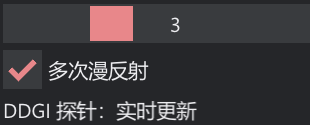
\includegraphics[width=.43\linewidth]{figures/probe-controls.png}\hspace{.04\linewidth}

\includegraphics[width=.43\linewidth]{../../../output/profiling/point-materials/bathroom-reopened.png}\\[-1pt]
{\small 浴室实拍。左图记录早期的实时模式；右图在点光源更新后重新烘焙，退出并重开后显示「已烘焙」。}
\end{center}

每个方向留下两个四维向量。第一组的前三项是红、绿、蓝的间接光，第二组的前两项是命中距离及其平方的平均。沿用着色器的存法，两组共占 32 字节。整间房有 $12\times6\times7\times6=3\,024$ 组方向记录，合计 96\,768 字节，加上文件头共 96\,792 字节。浴室的文件名是 \texttt{RTXGI-Bathroom.redflag.rfprobes}。

重新打开场景时，程序把模型三角形、材质、贴图和点光源与烘焙时的记录核对。相符的探针直接传回显卡。接着照常为眼前的像素寻找附近的探针，移动相机、改变面板大小都可以继续用这份数据。把柜门换成另一种颜色或移走窗边灯，旧数据就失去了依据。面板会切回「实时更新」，此时再烘焙一次即可。

\noindent{\small\color{quiet}C++ 接口调用示例\quad\href{run:../../Redflag/src/Redflag/Renderer/GI/GlobalIllumination.cpp}{\texttt{GlobalIllumination.cpp}}}\par\nopagebreak
\begin{lstlisting}[escapeinside={(*@}{@*)}]
gi.SetLights(sceneLights);
gi.BakeProbes(file);  (*@{\footnotesize\color{quiet}// 把房间各处收到的反射光写入场景旁的文件。}@*)

(*@{\footnotesize\color{quiet}// 下次打开后，先按场景恢复模型与点光源，再尝试读回上次的结果。}@*)
bool ready = gi.LoadProbes(file);
gi.Render(GIMethod::DDGI);  (*@{\footnotesize\color{quiet}// 如果上次的光照已过期，这一帧会重新计算探针。}@*)
\end{lstlisting}

在 Sponza 固定机位，先从一个进程输出 $160\times90$ 的间接光，再退出并用第二个进程加载文件。两张图全部 14\,400 个 HDR 像素逐字节相同。浴室还多试了一步，烘焙后按 Ctrl+S 再退出。场景文件把三盏灯按相反顺序写回去，重新打开仍显示「已烘焙」。点光源排列顺序可以改变，位置、强度、颜色和影响半径都参与核对。RenderDoc 里保留了给表面插值的计算，省掉了更新探针的一遍。\href{run:Redflag-Rendering-Performance.pdf}{《渲染性能实测》}

\clearpage
\section{ReSTIR DI 的选灯与复用}
\label{lesson-restir-di}
% 前置知识
从正在画的石柱向一盏灯发阴影光线，才知道这束光有没有被栏杆挡住。若逐像素枚举所有灯，代价随灯数增加。两盏灯的例子给了另一条路，先随机找候选，再让比较亮的候选更有机会留下来。一个蓄水池 \term{reservoir} 只存一个候选，还存它代表过多少候选、累计过多少权重。这样即使一盏灯最后没留下，它的贡献也参与了选择概率。

% 公式推导
两个候选权重分别为 1 和 3。第一项必选，第二项到来时以 $3/(1+3)$ 的概率替换第一项，最终保存两者的概率是 $1/4,3/4$。这个过程可扩展到任意长的输入流。候选由概率 $q$ 提出，我们用标量亮度 $\hat p$ 作筛选目标，因此先令权重 $w=\hat p/q$。最终输出还要恢复彩色贡献并补偿选中的概率，否则偏爱亮灯会让画面变亮。

% 公式
记最终选中的灯为 $y$，候选数为 $M$，则
\[
  S=\sum_i w_i,\qquad W=\frac{S}{M\hat p(y)},\qquad L_o=f_{\rm RGB}(y)W.
\]
合并另一个蓄水池时，把它所代表的候选数带进来。本像素重新计算 $\hat p_x(y)$，加入的权重为 $\hat p_x(y)W_{\rm old}M_{\rm old}$。在新像素重新查遮挡，能识别邻居看到而自己看不到的灯。截断历史、过滤邻居都会改变采样性质，需要用基准检查偏差。
\pair{profiling/gi/direct-1spp.png}{每像素随机挑一盏灯}{profiling/gi/restir-di.png}{历史及邻居参与选择后的第八帧}
\clearpage
% 逐行伪代码
\subsection{把相邻像素选中的灯留下来}
\noindent{\small\color{quiet}按 GLSL 整理的伪代码\quad\href{run:../../Redflag/src/Redflag/Renderer/GI/Shaders/GI.comp}{\texttt{GI.comp}}}\par\nopagebreak
\begin{lstlisting}[escapeinside={(*@}{@*)}]
fresh = pickUniformLight(pixel)
neighbors = compatibleFreshNeighbors(pixel, count=4)
for r in [fresh, previousPixelReservoir, neighbors]:
    m = min(r.candidateCount, 16)
    totalCount += m
    target = luminance(directRGB(pixel, r.light))
    (*@{\footnotesize\color{quiet}旧池的样本回到当前表面，要重新计算它在这里的亮度。}@*)
    w = target * r.W * m
    sum += w
    if w > 0 and random() * sum < w:
        selected, selectedTarget = r, target
W = sum / (totalCount * selectedTarget) if selectedTarget > 0 else 0
writeHistory(selected, W, totalCount)
output = directRGB(pixel, selected.light) * W
\end{lstlisting}
全黑时留空蓄水池并返回零。程序分两次调度，先让所有像素产生自己的新候选，第二次才读邻居。这样一个像素不会读到另一个像素写了一半的结果。NVIDIA 的 MinimalSample 把获取场景表面和光源的工作交给应用，复用代码单独存放。这里直接在同一份 GLSL 中读取点光源数组。每像素每帧只提一个新候选，让我们能数清借用邻居前后实际多查了几束影子。\href{https://github.com/NVIDIA-RTX/RTXDI/blob/main/Doc/Integration.md}{RTXDI 集成指南}

四个邻居决定每像素最多额外检查几处光路。兼容条件中的法线点积阈值 0.85 对应夹角约 $32^\circ$，位置距离 0.8 则相当于这个归一化场景最大跨度的 4\%。它们是阻止跨墙借样本的几何筛选。旧池的候选数另限为 16，作用是限制它在新选择中占的权重；调高后旧光照也会保留更久。

% 接口与数据结构
\begin{fields}
\texttt{Reservoir.y.w} & 直接光模式下是灯号。正式场景用本像素的金属度、粗糙度、底色和阴影重新计算 RGB 与选择权重。\\
\texttt{stats.x, stats.y} & 保存 $W$ 和候选数，分别由 \texttt{mergeR} 与下一帧历史读取。\\
\texttt{ReSTIRDI} & 当前每帧每像素提出一个新候选，读旧帧同一像素与最多四个邻居。相机大幅改变时需处理历史有效性。\\
\end{fields}

% 验证标准
在 Sponza 的 16 盏灯纯漫反射对照中，四个种子的平均 MSE 从独立 1 spp 的 \measured{direct-1spp-mse} 降到第八帧的 \measured{restir-di-mse}。花相同的八个新候选做独立平均得到 \measured{direct-8spp-mse}。三者的邻居访问和阴影射线工作量不同。亮度为正的像素中有 \measured{restir-di-reused_fraction_positive}\% 选中了复用样本；若以全部可见像素为分母则为 \measured{restir-di-reused_fraction_visible}\%。这两个比例回答不同的问题。

\par\noindent{\small\color{quiet}材料索引\enspace \href{https://github.com/NVIDIA-RTX/RTXDI}{RTXDI 集成代码}\enspace · \enspace \href{https://github.com/NVIDIA-RTX/RTXDI/blob/main/Doc/Integration.md}{NVIDIA 的集成指南}\enspace · \enspace \href{https://doi.org/10.1145/3386569.3392481}{论文 DOI 10.1145/3386569.3392481}\enspace · \enspace \href{https://intro-to-restir.cwyman.org/}{SIGGRAPH 的 ReSTIR 入门课}\enspace · \enspace \href{https://pbr-book.org/4ed/Monte_Carlo_Integration/Improving_Efficiency}{PBRT 提高采样效率}\enspace · \enspace \href{run:../../docs/latex/lighting/restir-di.tex}{可编辑笔记}}
\clearpage
\section{ReSTIR GI 的二次交点}
\label{lesson-restir-gi}
% 前置知识
直接光只需写下“选中第几盏灯”。间接光要写下“这条光线先碰到了哪里”。设地板上的点为 $x$，柱子上的点为 $y$。柱子受到灯光照射，再把光反射到地板。邻近像素 $x'$ 可以尝试连接同一个 $y$。改变起点后，距离、两端的夹角和中间有没有障碍都可能变化，只复制旧像素的颜色会忽略这三件事。

\begin{center}
\begin{tikzpicture}[x=.90cm,y=.86cm,font=\small]
  \fill[fill=shade,rounded corners=3pt] (0,0) rectangle (15.6,3.6);
  \fill[quiet!20] (1.1,.65) rectangle (1.45,2.95);
  \fill[quiet!20] (1.1,.48) rectangle (8.65,.65);
  \fill[quiet!62] (3.05,.65) rectangle (3.35,1.48);
  \coordinate (y) at (1.45,2.65);
  \coordinate (x) at (7.55,.65);
  \coordinate (near) at (4.35,.65);
  \draw[->,teal!70!black,very thick,shorten >=2pt] (x)--(y);
  \draw[wine,very thick] (near)--(3.35,1.34);
  \draw[wine,densely dashed] (3.35,1.34)--(y);
  \foreach \p in {x,near,y} \fill[ink] (\p) circle[radius=2pt];
  \node[anchor=south west] at (1.5,2.65) {柱上的反射点 $y$};
  \node[anchor=north] at (7.55,.55) {$x$};
  \node[anchor=north] at (4.35,.55) {$x'$};
  \draw[quiet!45] (8.94,.45)--(8.94,3.1);
  \node[anchor=west,text=teal!70!black] at (9.25,2.56) {从地板上的 $x$ 能看见 $y$。};
  \node[anchor=west,text=wine] at (9.25,1.76) {相邻点 $x'$ 的视线被挡住，};
  \node[anchor=west] at (9.25,1.08) {这条路径的贡献为零。};
\end{tikzpicture}\\[1pt]
{\footnotesize\color{quiet}本册绘制的侧面图。两条线都连向同一个反射点，灰色小块是地上的遮挡物。}
\end{center}

% 公式推导
从 $x$ 望向 $y$，同一块小纸片离得越远，占视野的角度越小。若纸片实际面积是 $dA$，斜着看时有效投影还要乘上纸片法线与观察方向的余弦。它张开的立体角是 $d\omega=(n_y\cdot-\omega)_+\,dA/r^2$。这里的比例就是换变量用到的雅可比 \term{Jacobian}。把一块正对眼睛、面积约 0.01 的小片从距离 1 移到 2，它占的立体角大约由 0.01 变成 0.0025 球面度。PBRT 的概率换元和 GAMES101 的点积在这里进入同一个式子。

% 公式
令 $\omega=(y-x)/r$，$c_x=(n_x\cdot\omega)_+$，$c_y=(n_y\cdot-\omega)_+$。对从 $x$ 按余弦取样得到的二次点，
\[
 p_A(y)=\frac{c_xc_y}{\pi r^2},\qquad
 f_A(x,y)=\frac{\rho_x}{\pi} L_o(y)\,\frac{c_xc_y}{r^2}\,V(x,y).
\]
概率和贡献都按每单位面积定义。复用时在新起点算 $f_A(x',y)$；它和旧池中的 $W$ 配合。若贡献用面积，提议概率却仍用每单位立体角，距离翻倍时就会得到错误的权重。
\pair{profiling/gi/indirect-8spp.png}{单像素独立积累八个样本}{profiling/gi/restir-gi.png}{一次反弹的 ReSTIR GI}
\clearpage
% 逐行伪代码
\subsection{重新连接柱子上的反射点}
\noindent{\small\color{quiet}按 GLSL 整理的伪代码\quad\href{run:../../Redflag/src/Redflag/Renderer/GI/Shaders/GI.comp}{\texttt{GI.comp}}}\par\nopagebreak
\begin{lstlisting}[escapeinside={(*@}{@*)}]
direction = cosineSample(normalAt(x))
y = trace(x, direction)
if hit(y):
    radianceAtY = estimateDirectLight(y)
    pdfArea = cosineAtX * cosineAtY / (pi * distanceSquared)
    candidate = (y.position, y.normal, radianceAtY, 1 / pdfArea)
for r in compatibleCandidates:
    (*@{\footnotesize\color{quiet}试着从脚下连到柱面，中途撞墙就去掉这条路径。}@*)
    visibility = traceSegment(x, r.y)
    targetRGB = albedo(x) * r.radiance * geometry(x, r.y) * visibility / pi
    mergeReservoir(r, luminance(targetRGB))
output = evaluateSelectedAt(x) * selectedWeight
\end{lstlisting}
一条新射线已经确认过 $x$ 到 $y$ 可达。对邻居和历史候选重新连线时必须再查遮挡；保存亮度较大的候选也不能穿墙。没命中二次表面、没有灯或背面余弦为零时，该候选贡献为零。

在 NVIDIA 的 GI 集成中，调用者提供第二个表面的位置、法线、原射线的取样密度，以及从那里回来的亮度。Redflag 在柱面均匀抽一盏点光源估计这份亮度，路径就此结束。PBRT 的路径追踪器还可以在柱上继续选方向，经过更多表面，适合用来研究多次反弹。\href{https://github.com/NVIDIA-RTX/RTXDI/blob/main/Doc/RestirGI.md}{NVIDIA 的 GI 集成说明}\quad\href{https://pbr-book.org/4ed/Light_Transport_I_Surface_Reflection/A_Better_Path_Tracer}{PBRT 第四版 §13.4}

% 接口与数据结构
\begin{fields}
\texttt{Reservoir.y, ny} & 世界空间二次交点及其法线；决定邻居重连时的方向、距离与背面剔除。\\
\texttt{Reservoir.lo} & 二次点处估计的出射光，来自实际点光源和遮挡查询。\\
\texttt{Render(ReSTIRGI)} & 读写两份历史蓄水池和一份当前帧候选。当前位置和法线来自公共可见表面数组。\\
\end{fields}

% 验证标准
间接光参考平均了两组互相独立的 512 spp。独立 1 spp、独立 8 spp 和 ReSTIR GI 第八帧的 MSE 分别为 \measured{indirect-1spp-mse}、\measured{indirect-8spp-mse} 和 \measured{restir-gi-mse}。第八帧有 \measured{restir-gi-reused_fraction_visible}\% 的可见像素选中了历史或邻居的候选。这组固定相机读数检验的是不透明漫反射材质的一次反弹。动态蒙皮和更多次反弹还需要各自的参考图。

\par\noindent{\small\color{quiet}材料索引\enspace \href{https://github.com/NVIDIA-RTX/RTXDI/blob/main/Doc/RestirGI.md}{RTXDI 的 GI 集成}\enspace · \enspace \href{https://doi.org/10.1111/cgf.14378}{论文 DOI 10.1111/cgf.14378}\enspace · \enspace \href{https://intro-to-restir.cwyman.org/}{ReSTIR 课程讲义}\enspace · \enspace \href{https://pbr-book.org/4ed/Monte_Carlo_Integration/Transforming_between_Distributions}{PBRT 概率换元}\enspace · \enspace \href{https://pbr-book.org/4ed/Light_Transport_I_Surface_Reflection/A_Better_Path_Tracer}{PBRT 第四版 §13.4 路径追踪}\enspace · \enspace \href{run:../../docs/latex/lighting/restir-gi.tex}{可编辑笔记}}
\clearpage
\section{GTAO 的遮挡轮廓}
\label{lesson-gtao}
% 前置知识
龙身在地上投出一道向右延伸的长影。换成右图，长影的位置几乎是白的，龙爪贴地的地方却有几小块深灰。长影只要挡住从点光源射来的那束光就能形成；紧挨龙爪的地面向四周望去，有好几个方向都被龙身挡住了。GTAO 要估算的，就是每块表面还能从哪些方向收到环境光。

\begin{center}
\begin{minipage}{.48\linewidth}\centering
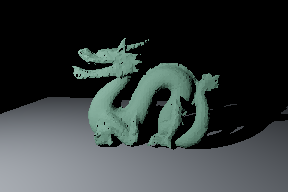
\includegraphics[width=\linewidth]{figures/dragon-direct.png}\\[-1pt]
{\small 点光源照出的龙与投影}
\end{minipage}\hfill
\begin{minipage}{.48\linewidth}\centering
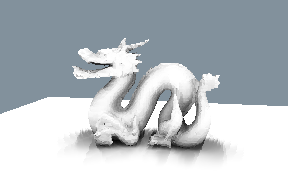
\includegraphics[width=\linewidth]{figures/dragon-visibility.png}\\[-1pt]
{\small GTAO 可见度，白色为 1，黑色为 0}
\end{minipage}\\[4pt]
{\footnotesize\color{quiet}Stanford Dragon，Redflag Vulkan，同一机位的 $288\times192$ 输出。蓝灰色区域没有模型。}
\end{center}

相机看向龙爪边的地面，深度图只记录每个像素最先看到的表面。LearnOpenGL 的 SSAO 教程在这一点周围取样，对照深度图估计有多少处被遮住。GTAO 仍然用到这些表面，但会沿几个方向分别寻找遮挡物的轮廓。想象用一张竖纸同时切过相机和地板上的点，龙爪便在纸上留下一条轮廓线。把这张纸绕观察方向转几次，每次找到轮廓的最高处，就能估计表面总共还能看到多大一片天空。

% 公式推导
沿刚才的纸面来看这小块地板。取从地板指向相机的单位方向 $v$，截面上与 $v$ 垂直的单位向量 $t$。纸面上任一入射方向可写成 $\omega=v\cos u+t\sin u$，其中 $u$ 从相机方向开始量。法线 $n$ 受光的余弦是 $n\cdot\omega$，球面上这段圆弧对应的面积还含 $\sin u$。可见弧从 $0$ 延伸到遮挡角 $h$，也要在法线所在半球的边缘停下。找到遮挡轮廓后，剩下这段积分就能直接算出。

% 公式
设 $a=n\cdot v,\ b=n\cdot t$，单侧截面的照明贡献为
\[
  I(h)=\int_0^h(a\cos u+b\sin u)\sin u\,du
      =\frac{a}{2}\sin^2 h+b\left(\frac h2-\frac{\sin(2h)}4\right).
\]
若地板正对观察者，$a=1,b=0$。无遮挡时 $h=\pi/2$，每侧贡献 0.5，两侧正好得到一整份可见度。$h$ 降到 $\pi/4$，这一侧贡献就降到 0.25。这个例子能检查半球归一化的系数。
\clearpage
% 逐行伪代码
\subsection{在深度图上寻找遮挡}
\noindent{\small\color{quiet}按 GLSL 整理的伪代码\quad\href{run:../../Redflag/src/Redflag/Renderer/ScreenSpace/Shaders/GTAO.comp}{\texttt{GTAO.comp}}}\par\nopagebreak
\begin{lstlisting}[escapeinside={(*@}{@*)}]
blocked = 0
for slice in fourDirectionsAtThisPixel:
    for side in [left, right]:
        h = angleWhereThisSideLeavesNormalHemisphere()
        for distance in eightDistancesWithinRadius:
            neighbor = nearestSurfaceAt(project(point + tangent * distance))
            if neighbor is above the surface and inside radius:
                next = angleBetween(view, neighbor - point)
                if next < h:
                    (*@{\footnotesize\color{quiet}只扣掉两条轮廓之间新增的那段遮挡。}@*)
                    blocked += (I(h) - I(next)) * weight(length(neighbor-point))
                    h = next
visibility = clamp(1 - blocked / 4, 0, 1)
\end{lstlisting}
箱子前面的地面向四周收光。在同一截面上，近处箱沿已经遮住一段圆弧，远处柱子可能挡住另一段。半径为 $r$ 时，前 $0.6r$ 内的样点保留全部遮挡，之后用平滑曲线减弱，到 $r$ 时权重为零。每次只给新挡住的那段弧乘距离权重。如果让远处的样点把整条轮廓一起淡出，紧贴箱壁的地面也容易过亮。

默认 $r=0.65$ 个场景单位，按米建模时就是 65 厘米。一个像素量四个截面，每侧查看八个位置。四个相邻像素稍微转动各自的截面，合在一起能量到十六个方向。\texttt{GTAOFilter.comp} 在周围 $3\times3$ 个像素里按离中心的远近取平均。箱壁和地面的法线相差约 $90^\circ$，两边各自取平均，柱脚的边缘便能留下来。最后再应用面板里的遮蔽强度，将结果乘到环境光上。

% 接口与数据结构
\begin{fields}
\texttt{GISurface} & 可见表面的世界位置、法线和底色。当前实现直接读世界位置，省去从深度图还原位置的一步。\\
\texttt{AORadius} & 世界单位。半径越大越能看到远处遮挡物，固定八步也会变得更稀。\\
\texttt{AOIntensity} & 对可见度施加指数。输出第四通道保留遮蔽系数，可把它只乘在间接漫反射上。\\
\end{fields}

在 Sponza 将半径缩到 0.0001，旧版固定方向采样的平均可见度从 \measured{ao_mean} 变为 \measured{ao_negligible_radius_mean}。镜头外的柱子无法出现在这份表面图里，也不能投下屏幕空间遮蔽。移动相机的实测和局部放大图见《渲染性能实测》的“移动相机下的柱脚遮蔽”。

可见弧积分见 Jimenez 等人的技术报告第 2 节。Intel 的 XeGTAO 实现说明也介绍了半球射线参考与邻域过滤。

\par\noindent{\small\color{quiet}材料索引\enspace \href{https://github.com/GameTechDev/XeGTAO}{Intel XeGTAO}\enspace · \enspace \href{https://www.activision.com/cdn/research/PracticalRealtimeStrategiesTRfinal.pdf}{Activision 技术报告}\enspace · \enspace \href{https://blog.selfshadow.com/publications/s2016-shading-course/activision/s2016_pbs_activision_occlusion.pdf}{SIGGRAPH 2016 讲义}\enspace · \enspace \href{https://learnopengl.com/Advanced-Lighting/SSAO}{LearnOpenGL 的 SSAO}\enspace · \enspace \href{run:../../docs/latex/lighting/gtao.tex}{可编辑笔记}}
\clearpage
\section{TAA 的采样位置与重投影}
\label{lesson-taa}
% 前置知识
在石柱的斜边上，一个像素可能一半覆盖石头、一半覆盖背景。本帧只在中心取一个点，下一帧把采样点挪开一点，便能观察到不同的覆盖情况。这些观测可以积累到一起，条件是找回同一块石头在上一帧的位置。GAMES101 的模型、观察和投影变换，以及 RTR4 附录里的透视除法，正好就是这里要用的工具。

% 公式推导
可见表面已经给出世界坐标 $p=(x,y,z,1)$。乘上偏移前的观察投影矩阵得到齐次坐标 $c$，除以 $c_w$ 后才是屏幕位置。用两帧的相机分别投影同一个点，就能分清“相机移动了多少”和“这次在像素内取了哪个样本”。若相机静止，旧颜色就存在同一显示像素。若相机真在移动，旧位置通常落在四个像素之间，此时才做双线性插值，并检查那里以前是否被别的柱子挡住。

% 公式
记视口宽高为 $(W,H)$，原点在左上。$s(c)$ 把齐次位置换算为像素，$i$ 是当前整数像素中心。运动矢量用两个偏移前的投影相减，所以半像素的中心约定也随之抵消。
\[
 s(c)=\left(\tfrac12+\tfrac12c_x/c_w,\ \tfrac12-\tfrac12c_y/c_w\right)(W,H),\quad
 q=i+s(c_{t-1})-s(c_t).
\]
找到旧位置以后，还要检查旧图里画的是不是同一面墙。设投影矩阵把观察坐标的高度乘以 $P_{yy}$，画面高 $H$ 像素。一个像素在标准化坐标中高 $2/H$，把透视除法和高度缩放倒过来，就得到它在墙面深度处对应的世界高度 $h=2w/(|P_{yy}|H)$。透视相机的 $w$ 是沿视线轴量出的深度，远墙的一个像素盖得更宽；正交相机的 $w=1$，同一面墙退远后仍占相同像素数。旧点与眼前的点若相距超过 $2.5h$，这里就舍掉旧颜色。2.5 是经验值，取大了容易把前景颜色拖到背后的墙上，取小了则会丢掉本可用的历史。

像素最后得到 $C=(1-\alpha)C_t+\alpha C_{t-1}$。镜头停住后，如果同一个像素先采到栏杆、又采到后面的墙，就按实际采样次数混色。已有 $n$ 次采样时取 $\alpha=n/(n+1)$，这样第 $n+1$ 次和前面每一次各占相同的一份。其余像素仍受用户设置的历史权重上限控制。移动镜头时，每块表面回到上一帧的位置各不相同，引擎会舍去已经混入两层表面的旧颜色。剩下四个邻居中，通过检查的插值权重之和若为 0.5，历史占比就再减半。
\pair{screen-effects/taa.png}{静止八帧后的颜色}{screen-effects/taa-history.png}{横移相机后，亮处仍能采用旧帧}
\clearpage
% 逐行伪代码
\subsection{找回上一帧的颜色}
\noindent{\small\color{quiet}按 GLSL 与相机代码整理的伪代码\quad\href{run:../../Redflag/src/Redflag/Renderer/ScreenSpace/Shaders/TAA.comp}{\texttt{TAA.comp}}}\par\nopagebreak
\begin{lstlisting}[escapeinside={(*@}{@*)}]
jitter = centeredSample16[frame % 16]
if (frame / 16) % 2 == 1:
    jitter = (-jitter.y, jitter.x)
projection = shiftClipPositionByPixelFraction(projection, jitter)
drawVisibleSurfacesAndColor(projection)
if cameraIsStill and sceneHasNotChanged:
    if sampledTwoSurfaces and historyWeight > 0:
        weight = previousStillSamples / (previousStillSamples + 1)
    return blend(current, history[pixel], weight)
motion = previousStablePixel(world) - currentStablePixel(world)
(*@{\footnotesize\color{quiet}加上运动量才得到旧图里的位置。}@*)
oldPixel = pixel + motion
pixelHeight = 2 * currentClip.w / (abs(projection.yy) * imageHeight)
for neighbor, coefficient in bilinearNeighbors(oldPixel):
    if validOldPosition(neighbor) and distanceToOldPoint(neighbor) <= 2.5 * pixelHeight:
        sum += coefficient * oldColor[neighbor]
        accepted += coefficient
if accepted > 0:
    old = clamp(sum / accepted, minRGB3x3, maxRGB3x3)
    current = mix(current, old, historyWeight * accepted)
writeSeparateHistory(currentColor, currentWorldPosition)
\end{lstlisting}

% 接口与数据结构
\begin{fields}
\texttt{JitterProjection} & 用偏移后的投影画几何。调用 \texttt{Render} 时再传偏移前的 \texttt{stableProjection}，用来计算相机运动。\\
\texttt{History[2], Positions[2]} & 每帧读一组、写另一组，下一帧换角色。颜色与世界位置必须来自同一帧。\\
\texttt{ResetHistory()} & 切场景、重建视口或跳切后，第一帧直接写新颜色。移动相机时仍可重投影静态物体。\\
\end{fields}

% 验证标准
用同一静态场景的八张抖动图求逐像素均值作对照。它代表这八个实际采样位置。检查 TAA 第一帧与当前输入逐像素相同；再侧移相机，刚露出的区域应拒绝历史。现阶段世界位置能处理静止几何上的相机运动，蒙皮或独立移动物体还需要它们自己的上一帧位置与运动向量。

早期八帧测试中，最后一张单帧与八张均值的 MSE 为 \measured{single_frame_vs_eight_jitters_mse}，混合后为 \measured{taa_vs_eight_jitters_mse}。另一组测试把红板放在蓝墙前，横移并旋转相机。正交视图中新露出的 54 个像素原先都混入红色，修正后误收为零；透视视图中新露出的 96 个像素在修改前后都正确。\href{run:../../output/profiling/taa-camera/fixed/measurements.csv}{逐项结果}

相机和场景都没动时，编辑器仍让 TAA 合并多帧的颜色。画满 32 帧，面板就一直显示最后一张图。这里的 32 决定显卡要多画多久，程序没有逐帧测量噪点，也就不能据此判断所有场景都已足够平滑。再移动相机、调灯或改变效果，面板会重新绘制。

\par\noindent{\small\color{quiet}材料索引\enspace \href{https://github.com/Unity-Technologies/Graphics/blob/master/Packages/com.unity.render-pipelines.universal/Shaders/PostProcessing/TemporalAA.shader}{Unity URP 源码}\enspace · \enspace \href{https://doi.org/10.1111/cgf.14018}{综述 DOI 10.1111/cgf.14018}\enspace · \enspace \href{https://advances.realtimerendering.com/s2014/}{Karis，SIGGRAPH 2014}\enspace · \enspace \href{https://sites.cs.ucsb.edu/~lingqi/teaching/resources/GAMES101_Lecture_04.pdf}{GAMES101 变换}\enspace · \enspace \href{https://www.realtimerendering.com/Real-Time_Rendering_4th-Appendices.pdf}{RTR4 附录 A}\enspace · \enspace \href{run:../../docs/latex/lighting/taa.tex}{可编辑笔记}}
\clearpage
\section{分簇筛选点光源}
\label{lesson-cluster}
% 前置知识
走廊近处和拱门后面各有一盏灯。若给每个像素都遍历场景里所有点光源，很多次计算都会得到零。LearnOpenGL 的延迟着色一章先算点光源的有效半径；把球形照明范围和相机的观察空间联系起来，就能在逐像素着色前先筛一次。这里先切 $16\times16$ 像素的小块，再把每块从近到远分为 16 段。每小段空间称为灯簇 \term{cluster}。

% 公式推导
相机看近处时，一米长的物体可能占满屏幕；放到远处就只占几个像素。按固定比率增加分段深度，近处自然得到更细的分段。若近端为 $n$、远端为 $f$、共 $K$ 段，要求 $n r^K=f$，解得 $r=(f/n)^{1/K}$。给定像素的相机深度 $z$，对深度比取对数就能找回它属于第几段。再检查哪盏灯的球与这段空间相交，把灯号写进表里。

% 公式
\[
 z_k=n(f/n)^{k/K},\qquad
 k=\operatorname{clamp}\!\left(\left\lfloor K\frac{\log(z/n)}{\log(f/n)}\right\rfloor,0,K-1\right).
\]
灯簇的八个角确定相机空间中的包围盒。将灯心 $l$ 的各坐标限制在盒子的范围，得到盒上最近点 $b$。若 $\|l-b\|^2\le R^2$，保留这盏灯。盒子包得稍大只会多留几盏，少留一盏则会让本该亮的地板变暗。
\pair{screen-effects/clustered.png}{49 盏灯的纯漫反射教学对照}{screen-effects/cluster-candidates.png}{每个像素要检查的灯数，白色代表 49}
\clearpage
% 逐行伪代码
\subsection{留下能照进这一簇的灯}
\noindent{\small\color{quiet}按 GLSL 整理的伪代码\quad\href{run:../../Redflag/src/Redflag/Renderer/ScreenSpace/Shaders/ClusterCull.comp}{\texttt{ClusterCull.comp}}}\par\nopagebreak
\begin{lstlisting}[escapeinside={(*@}{@*)}]
for cluster in tiles * depthSlices:
    box = cameraSpaceBoxOfEightCorners(cluster)
    for groupOf32Lights:
        mask = 0
        for light in groupOf32Lights:
            if distance(light.center, box) <= light.range:
                (*@{\footnotesize\color{quiet}第几个灯球碰到格子，就把整数里的第几位置为一。}@*)
                mask |= 1 << light.localIndex
        store(cluster, group, mask)
for pixel in visibleSurfaces:
    cluster = index(tileAt(pixel), sliceAt(viewDepth(pixel)))
    for light in setBits(masks[cluster]):
        if visible(pixel, light):
            color += reflectedPointLight(pixel, light)
\end{lstlisting}
一个无符号整数用 32 个比特表示 32 盏灯；第 33 盏从第二个整数的最低位开始。查表时只遍历值为 1 的位。片段仍须算真实距离和余弦，筛选阶段只知道灯可能有贡献。

$16\times16$ 是每个小块的像素尺寸。改成 $8\times8$ 时，同一画面大约需要四倍数量的灯表，但每块里可以少留一些无关的灯。当前对数分段参考深度从 0.05 到 250，两端的簇还包住更近和更远的表面。测试里的灯半径 4 是光照定义本身，CPU 逐灯对照和 GPU 必须使用同一个值。

% 接口与数据结构
\begin{fields}
\texttt{GILight} & 灯心先变到相机坐标与包围盒比较。下面实际着色时仍可在世界坐标算光照。\\
\texttt{Masks} & 一维无符号整数数组，长度为簇数乘 $\lceil\text{灯数}/32\rceil$，零灯也保留一个空字。\\
\texttt{Intensity.w} & 每盏灯在世界坐标中的影响半径。从编辑器的点光源属性调整，灯簇先用它筛选，着色再用它算衰减。\\
\end{fields}

% 验证标准
历史基准用纯漫反射，并关闭阴影来单独检查分簇。挑 49 盏灯是为了跨过一个整数能表示的 32 盏。测试使用相同半径和衰减公式在 CPU 端逐灯计算，比较每个像素的 RGB；把所有灯移除后，所有输出都应为零。使用 $161\times91$ 的画面还能验证右侧和底部的残缺小块。减少候选数量衡量筛选效率，能否减少整帧耗时还取决于建表成本。

可见像素平均需检查 \measured{cluster_mean_candidates} 盏灯；与逐灯参考之间最大的 RGB 分量绝对误差为 \measured{cluster_max_absolute_rgb_error}。

\par\noindent{\small\color{quiet}材料索引\enspace \href{https://github.com/google/filament/blob/main/filament/src/Froxelizer.cpp}{Filament 的 Froxelizer}\enspace · \enspace \href{https://doi.org/10.2312/EGGH/HPG12/087-096}{HPG 论文 DOI 10.2312/EGGH/HPG12/087-096}\enspace · \enspace \href{https://doi.org/10.1145/2343045.2343095}{SIGGRAPH 2012 报告}\enspace · \enspace \href{https://learnopengl.com/Advanced-Lighting/Deferred-Shading}{LearnOpenGL 延迟着色}\enspace · \enspace \href{run:../../docs/latex/lighting/cluster.tex}{可编辑笔记}}
\clearpage
\section{粗糙表面的随机屏幕反射}
\label{lesson-ssr}
% 前置知识
在抛光石地上能看到立柱的倒影。粗糙表面可以想象成许多朝向略有不同的小镜子，PBRT 和 LearnOpenGL 的微表面模型都从这个想法出发。理想镜面只有一条反射方向；粗糙材质则可以从一个分布里抽出一面小镜子的法线，再按镜面反射定律追踪它。当前帧的深度和颜色已提供一张可查询的表，便可沿反射线寻找屏幕上先被它遇到的表面。

% 公式推导
令 $v$ 为表面指向眼睛的方向，$h$ 为 GGX 分布抽到的微表面法线，$l$ 为反射方向。微表面越粗糙，$h$ 离几何法线 $n$ 越远的机会越大。方向采样的概率必须一起带进估计量。取半程向量的密度 $p_h=D(h)(n\cdot h)$，对于镜面反射换成出射方向后，$p_l=p_h/(4|v\cdot h|)$。这里的概率原本描述小镜子的朝向，实际追踪的却是反射光线，所以算权重前需要换元。

% 公式
若屏幕交点有入射光 $L_i$，反射贡献估计为 $L_i f_s(n\cdot l)/p_l$。代入微表面反射函数 $f_s=DFG/[4(n\cdot v)(n\cdot l)]$，消掉相同因子后得到
\[
 l=2(v\cdot h)h-v,\qquad
 L_{\rm refl}= L_i F\,G\,\frac{v\cdot h}{(n\cdot v)(n\cdot h)}.
\]
$F$ 是掠射角下更强的菲涅耳反射，$G$ 则考虑小镜面之间的相互遮挡。图中的早期实验令整块地面使用同一粗糙度，非金属取 $F_0=0.04$。编辑器的组合光照按像素读取粗糙度和金属度；SSR 找到画面里的物体时，倒影取该处像素的颜色。下一节会把灯牌放在相机身后，看看怎样把它也画进镜子。
\pair{screen-effects/ssr.png}{直接颜色加随机反射}{screen-effects/ssr-hits.png}{白点表示反射线找到了可见表面}
\clearpage
% 逐行伪代码
\subsection{沿反射线寻找屏幕交点}
\noindent{\small\color{quiet}按 GLSL 整理的伪代码\quad\href{run:../../Redflag/src/Redflag/Renderer/ScreenSpace/Shaders/StochasticSSR.comp}{\texttt{StochasticSSR.comp}}}\par\nopagebreak
\begin{lstlisting}[escapeinside={(*@}{@*)}]
u, phi = random2(pixelIndex, frame)
h = sampleGGXHalfVector(roughness, u, phi)
ray = reflect(-view, h)
for distance in increasingSteps(maxDistance, count=64):
    p = worldOrigin + ray * distance
    q = projectToScreen(p)
    if outside(q): break
    if behindVisibleSurface(p, q):
        (*@{\footnotesize\color{quiet}在刚刚穿过深度表面的这段路上折半，收紧交点位置。}@*)
        narrowIntervalFiveTimes()
        if closeInDepth and frontFacing and notSelfHit:
            output += sceneColor[hitPixel] * brdfWeight
        break
\end{lstlisting}
步数固定时，近处先用更密的步长。比较时双方都转换为相机前方的线性距离，不能直接拿一方的投影深度去减另一方的米数。五次二分查找收窄穿过深度的区间；命中厚度过宽会把无关的柱子当作反射源。

默认最远距离 12 使用场景世界单位，64 是每条射线的最大步数。局部找到相交区间后再折半五次，最终区间宽度是原来的 $1/32$。材质检查选 0.08 和 0.65 两档粗糙度，用意是让窄反射和散开的反射容易区别。它们是对照材质的输入，不是根据命中率倒算出来的参数。

% 接口与数据结构
\begin{fields}
\texttt{Roughness} & 粗糙度经平方得到 GGX 粗糙参数。它改变采样方向分布，粗糙度较大时单样本噪声也更明显。\\
\texttt{ReflectionDistance} & 光线最多走多远，使用场景世界单位。单独测试 SSR 时，找不到可见表面就保留输入颜色。\\
\texttt{Render(..., inputColor)} & 接收当前线性颜色和表面数据，返回含反射的独立缓冲。第四通道记录是否命中。\\
\end{fields}

% 验证标准
固定帧编号与输入，两次 GPU 运行需逐值相等。改变粗糙度应同时改变命中图或颜色。这组测试只使用屏幕上的数据。把被反射的物体转出画面后，就查不到它的颜色。AMD 的完整 SSSR 还使用分层深度、光线分类与降噪；本章的均匀预算和命中图让这些扩展可以单独验证。原始 SIGGRAPH 课程和配套 JCGT 射线遍历论文均未列 DOI。

这次固定粗糙度 0.08，命中比例为 \measured{ssr_hit_fraction}（1 代表全部命中）。两次同帧产生的最大逐值差为 \measured{ssr_repeat_max_difference}。

\par\noindent{\small\color{quiet}材料索引\enspace \href{https://github.com/GPUOpen-Effects/FidelityFX-SSSR}{AMD SSSR 源码}\enspace · \enspace \href{https://jcgt.org/published/0003/04/04/}{JCGT 屏幕空间射线论文}\enspace · \enspace \href{https://h3.gd/stochastic-ssr/}{Stachowiak 的 SIGGRAPH 课程}\enspace · \enspace \href{https://pbr-book.org/4ed/Reflection_Models/Roughness_Using_Microfacet_Theory}{PBRT 微表面理论}\enspace · \enspace \href{https://sites.cs.ucsb.edu/~lingqi/teaching/games202.html}{GAMES202 课件}\enspace · \enspace \href{run:../../docs/latex/lighting/ssr.tex}{可编辑笔记}}
\clearpage
\subsection{屏幕外的倒影}
\label{sec:mirror}

相机正对一面镜子，灯牌架在相机背后。打开 SSR，镜面上的像素可以沿反射方向去查本帧画好的颜色。但整张图里没有一个像素画过灯牌，屏幕上就无从查到它的条纹。要画出镜子里的灯牌，可以从这个像素对应的镜面位置出发，沿反射方向去找房间里实际摆放的物体。

\begin{center}
\begin{tikzpicture}[x=1cm,y=1cm,font=\small,>=stealth]
\foreach \k/\heading in {0/镜子看得到灯牌,1/挡板遮住灯牌}{
  \begin{scope}[xshift=\k*7.85cm]
  \filldraw[rounded corners=2mm,fill=shade!75,draw=quiet!30] (0,0) rectangle (7.55,4.9);
  \node[anchor=west,font=\bfseries] at (.23,4.56) {\heading};
  \draw[teal!70!black,line width=1.8pt] (.7,3.65)--(6.7,3.65);
  \node[anchor=south east,text=teal!60!black] at (6.65,3.65) {镜面};
  \fill[teal!70!black] (2.60,3.65) circle (2.1pt);
  \draw[quiet!60,dashed] (2.6,3.62)--(2.6,2.47);
  \node[text=quiet,anchor=north] at (2.6,2.48) {法线};
  \draw[ink,thick,->] (1.45,1.85)--(2.58,3.61);
  \fill[ink] (1.45,1.85) circle (2pt);
  \node[anchor=north east] at (1.65,1.83) {相机};
  \draw[wine,line width=3pt] (4.01,.77)--(5.03,.77);
  \node[text=wine,anchor=north] at (4.52,.72) {条纹灯牌};
  \ifnum\k=0
    \draw[wine,thick,->] (2.62,3.62)--(4.43,.79);
  \else
    \draw[quiet!55,dashed] (3.67,1.98)--(4.45,.78);
    \draw[quiet,line width=3pt] (3.31,1.98)--(4.14,1.98);
    \node[text=quiet,anchor=west] at (4.22,1.98) {挡板};
    \draw[wine,thick,->] (2.62,3.62)--(3.63,2.02);
  \fi
  \end{scope}
}
\end{tikzpicture}
\end{center}
{\small\color{quiet}项目绘制的俯视图。按程序查找物体的方向读箭头：黑线从相机走到镜面，红线从镜面走到第一个交点。右图的虚线表示挡板后面的路，灯牌在这里照不进镜子。\par}

先看左图。画一条垂直于镜面的线，标作单位法线 $n$。从相机走到镜面的单位方向记为 $d$。把 $d$ 分成两部分，一部分沿着镜面向右，另一部分垂直镜面向里。反射后仍向右走，原本向里的那部分要改成向外。这一部分是 $(d\cdot n)n$，从 $d$ 减去它一次只够把它消掉，再减一次才会反向。于是从镜面出发的方向为
\[
    r=d-2(d\cdot n)n .
\]
例如用“向右、远离镜面”作两个坐标方向，来路 $d=(0.6,-0.8)$ 就会变成 $r=(0.6,0.8)$。着色器里的 $v$ 从表面指向相机，正好与来路相反，因此理想镜面的代码是 \texttt{reflect(-v,n)}。粗糙度为零时，\texttt{sampleReflection} 每次都取这条方向。粗糙表面则按前文的 GGX 分布选取小镜子的法线 $h$，再求 \texttt{reflect(-v,h)}。采到的方向散开，灯条的轮廓也会变宽。\href{https://pbr-book.org/4ed/Reflection_Models/Specular_Reflection_and_Transmission}{PBRT 第四版 §9.3.3，图 9.6、9.7}

右图里，沿同一方向既能碰到挡板，也能碰到灯牌。把起点记为 $P$，离镜面 $t$ 个场景单位的点就是 $P+t\,r$。查找只走到设置中的反射距离，默认是 12 个场景单位。范围内各个不透明表面当中，最小的正数 $t$ 给出挡板。在这个交点取颜色，即使挡板完全是黑色，也要把黑色留在倒影里。用“颜色够不够亮”判断有没有碰到东西，会让远处的灯牌或天空穿过挡板。

方向还不能决定镜子有多亮。理想的白金属可以把这条方向上的光全部反回来。对于项目里的光滑非金属材质，正对表面时镜面反射约占入射光的 4\%，朝侧面看时这个比例会增大。着色器用菲涅耳项 $F$ 表示这个比例。镜子照到天空时，粗糙度为零就从环境图最清晰的那层取色，再乘 $F$。

在 \texttt{Mirror-Studio} 里，镜面位于 $z=0$。相机的水平位置是 $x=-0.62,\ z=3$，灯牌中心在 $x=1.75,\ z=4.8$。想象把灯牌移到镜后一样远的地方，虚像就在 $z=-4.8$。从相机向虚像画直线，走过全程的 $3/7.8$ 就会与镜面相交。交点的横向位置是 $-0.62+(1.75+0.62)\times3/7.8\approx0.29$。从这里往真实灯牌连线，走到 $z=2.55$ 时，横向位置约为 $1.07$。把挡板中心摆在这里，就能遮住镜中的灯条，同时给相机留出看镜面的视线。\href{run:../../RedflagForge/assets/scenes/Mirror-Studio.redflag}{示例场景}\quad\href{run:../../tests/check_scene_reflections.py}{挡板的位置与截帧}

\clearpage
\subsection{倒影中的颜色}

组合光照先算出相机能直接看到的物体颜色，再算倒影。能够从屏幕上查到立柱时，直接读立柱那个像素的颜色。打开「实时效果」里 SSR 下的「屏幕外反射」后，射线在屏幕上找不到交点，还可以查询房间里的三角形。CPU 在加载几何时已经把附近的三角形分组，给每组套上包围盒。GPU 从镜面出发，光线没穿过的盒子可以整组略过。这次计算沿用间接光照的这份场景数据。

\noindent{\small\color{quiet}按计算着色器整理的伪代码\quad
\href{run:../../Redflag/src/Redflag/Renderer/ScreenSpace/Shaders/StochasticSSR.comp}{\texttt{StochasticSSR.comp}，\texttt{main}}}\par\nopagebreak
\begin{lstlisting}[escapeinside={(*@}{@*)}]
r, weight = sampleReflection(normal, view, roughness)
if hitScreen(r):
    incoming = sceneColor[hitPixel]    (*@{\footnotesize\color{quiet}这个像素已经算过光照。}@*)
else if traceScene and hitScene(r):
    incoming = shade(hit, -r)          (*@{\footnotesize\color{quiet}从交点朝镜子看，算它送来的光。}@*)
else:
    return base + environmentReflection
return base + incoming * weight        (*@{\footnotesize\color{quiet}镜面把入射光中的这一份反射到相机。}@*)
\end{lstlisting}

镜子照到灯牌时，交点给出灯牌上的纹理坐标。顺着坐标找到发光贴图上的条纹，把纹素从 sRGB 转为线性颜色，再乘材质的发光颜色和强度，就能分清亮条、暗条和黑边。若照到一面普通墙，还要看哪些点光源或方向光能照到它。此时视线从墙指向镜子，高光的方向也按这条视线计算。启用 DDGI 后，墙面还能从附近的探针取到反射来的光。编辑器在探针算完第一轮或读入烘焙文件后才使用这份数据。镜子前什么都没碰到时，已启用的镜面环境光可以提供远景。环境图按方向取色，花纹随位置改变的近处灯牌需要前面的交点才能画准。

这些计算可在 \href{run:../../Redflag/src/Redflag/Renderer/ScreenSpace/Shaders/SceneReflection.glsl}{\texttt{SceneReflection.glsl} 的 \texttt{sceneReflection}} 中找到。交点取三角形本身的法线，法线贴图刻出的细纹可能在倒影里变平。计算会略过标成半透明的玻璃。若叶片使用透明度裁剪，射线会在交点读取贴图的透明度，遇到孔隙便继续查找后面的物体。镜子里出现第二面镜子时，只计算第二面镜子自身的材质和照明。

在 GPU 上读一次屏幕颜色很直接，沿场景查找还需读包围盒、三角形和材质。AMD 的 FidelityFX 示例也利用两种查询各自能看到的物体，并用屏幕分块和降噪控制工作量。本项目由 Vulkan 计算着色器沿包围盒查找，同一条反射光线找到屏幕颜色就结束查找。屏幕颜色来自主相机的视角，因此把带窄高光的物体转过屏幕边缘时，两种方法算出的高光仍可能不同。\href{https://gpuopen.com/manuals/fidelityfx_sdk/samples/hybrid-reflections/}{AMD 示例说明}\quad\href{https://github.com/GPUOpen-LibrariesAndSDKs/FidelityFX-SDK/blob/v1.1.4/samples/hybridreflections/shaders/Intersect.hlsl}{SDK 1.1.4 源码}\quad
\href{https://gpuopen.com/download/GDC_Performant_Reflective_Beauty_Hybrid_Ray_Traced_Reflections_In_Far_Cry_6.pdf}{GDC 2022 讲义，第 74--77 页}

\pair[.43\linewidth]{profiling/scene-reflections/bathroom-screen.png}{只开 SSR}{profiling/scene-reflections/bathroom-scene.png}{加上屏幕外反射}
{\small\color{quiet}RTXGI Bathroom 同机位，第 24 帧，RenderDoc 回放，$320\times205$。看洗手盆上方的圆镜：右图能看到身后墙砖的明暗交界，镜面和粗糙的地面仍有颗粒。\par}

\clearpage
\subsection{灯条与挡板的实测}

回到 \texttt{Mirror-Studio}，用相同机位捕获第 24 帧。左图里镜面上有两处点光源的高光，但灯牌没有出现。右图里多出三条橙色灯带，后方的墙也进入倒影。再把绿色挡板放到镜面和灯牌的连线上，镜子里原本最亮的区域就变成绿色。三次都保留 SSR，改动的是从场景中查找物体的开关和挡板的位置。

\pair{profiling/scene-reflections/mirror-screen.png}{仅从屏幕取色}{profiling/scene-reflections/mirror-scene.png}{从场景中找到灯牌}
\begin{center}
  \begin{minipage}[c]{.48\linewidth}\centering
    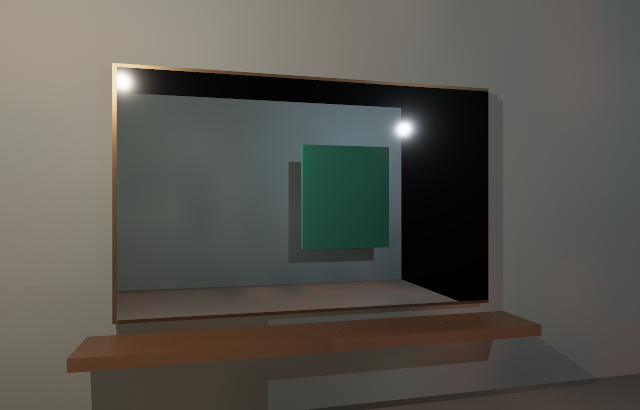
\includegraphics[width=\linewidth]{../../../output/profiling/scene-reflections/mirror-blocked.png}\\[-2pt]
    {\small 在镜子和灯牌之间放入挡板}
  \end{minipage}\hfill
  \begin{minipage}[c]{.48\linewidth}\centering
  {\small 加入屏幕外反射后，镜中各处的读数}\par\smallskip
  \small\begin{tabular}{@{}lrr@{}}
    \toprule 取样处 & 红通道 & 绿通道\\\midrule
    亮条中心 & \measured{mirror-white-r} & \measured{mirror-white-g}\\
    灰条中心 & \measured{mirror-gray-r} & \measured{mirror-gray-g}\\
    黑色间隔 & \measured{mirror-black-r} & \measured{mirror-black-g}\\
    绿色挡板 & \measured{mirror-board-r} & \measured{mirror-board-g}\\\bottomrule
  \end{tabular}
  \end{minipage}
\end{center}
{\small\color{quiet}RenderDoc 1.47 回放，$640\times410$，原图使用编辑器的亮度映射。表中每项取交点附近 $3\times3$ 个像素的中位数，读取反射计算前后的线性颜色之差，所以数值可以大于 1。最后一行仍取第一行的位置。\par}

灯牌中间那条在 8 位贴图里取的是灰色 128。把 sRGB 转回线性亮度，理论上它发出的光约为白色的 $0.216$ 倍。灯牌表面同时也会反射房间的光，可以用不发光的黑色间隔估计这部分。用上表的红通道扣除它，得到 $(\measured{mirror-gray-r}-\measured{mirror-black-r})/(\measured{mirror-white-r}-\measured{mirror-black-r})\approx\measured{mirror-stripe-ratio}$。这样既检查了射线找到的物体，也检查了取到哪条花纹、它应该有多亮。

只开 SSR 时，这三个位置的反射增量全部为零。放入挡板后，亮条原处的红通道降到 \measured{mirror-board-r}，绿通道仍有 \measured{mirror-board-g}，镜子收到了挡板送来的光。单帧可以看出颜色是否正确。要判断同一像素的亮度会不会来回跳动，还要把它在不同帧的值取出来比较。\href{run:../profiling/scene-reflections/frames.json}{五次截帧的图像、绘制事件与原始读数}
\clearpage
\subsection{理想镜面的边缘}

灯条的颜色对了，把镜中的灯牌放大，边缘却像撒着一层亮砂。相机和灯牌都没动，镜面材质的粗糙度也已经调到零。对于这样的镜面，表面法线和视线都固定，每帧应沿同一个方向取色。可以先查反射方向是否真的固定，再去调整 TAA。

\begin{center}\small
\begin{tabular}{@{}c@{\hspace{12mm}}c@{}}
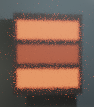
\includegraphics[width=.28\linewidth]{../../../output/profiling/scene-reflections/mirror-edge-before.png} &

\includegraphics[width=.28\linewidth]{../../../output/profiling/scene-reflections/mirror-edge-after.png}\\[-2pt]
旧版仍然随机选方向 & 粗糙度为零时用镜面方向
\end{tabular}\end{center}
{\small\color{quiet}从两次 RenderDoc 回放的同一屏幕位置裁出灯牌，各取第 24 帧的 $94\times107$ 个像素。两次都用粗糙度为零的镜子，使用同一份烘焙探针。可对照灯条内部和四边，亮砂主要出现在亮暗交界处。\par}

旧着色器用 $a=\max(0.002,\,\text{roughness}^2)$ 决定抽样范围。它本来用来画有粗糙度的材质。即使把粗糙度调到零，旧代码仍取 $a=0.002$，每帧抽出的小镜子朝向都会稍有变化。对着均匀墙面时，方向差一点，读出的颜色变化很小。到灯条的边上，光线稍偏就会从黑边打到亮条，或者从亮条打到黑边；接下来再混合几帧的颜色，两侧的颜色也会混在一起。

\noindent{\small\color{quiet}按 \href{run:../../Redflag/src/Redflag/Renderer/ScreenSpace/Shaders/StochasticSSR.comp}{\texttt{StochasticSSR.comp} 的 \texttt{sampleReflection}} 整理的伪代码}\par\nopagebreak
\begin{lstlisting}[escapeinside={(*@}{@*)}]
if roughness == 0:
    direction = reflect(-v, n)   (*@{\footnotesize\color{quiet}这一条方向正好符合镜面反射定律。}@*)
    weight = fresnel(dot(v, n))
else:
    h = sampleGGX(roughness)     (*@{\footnotesize\color{quiet}材质有粗糙度，才需要在不同方向取样。}@*)
    direction = reflect(-v, h)
    weight = microfacetWeight(v, n, h)
\end{lstlisting}

单独测试这项修改时，固定相机，在 $96\times96$ 的镜面上连续取 16 帧反射结果，跳过 TAA。以第一帧为准，每个像素的红、绿、蓝各有一个差值。将这三个差值的平方相加、开方，得到一次颜色变化的大小。取所有像素与帧中最大的那个，旧版是 4.031，新版为 0。这里比较的是送进后处理之前的浮点颜色，亮条自身的红通道就有 4，差值超过 1 也有实际意义。\href{run:../profiling/scene-reflections/test-stability.csv}{16 帧的比较记录}\quad\href{run:../../tests/SceneReflectionCheck.h}{测试中的灯条、挡板与镜面}

\clearpage
\subsection{粗糙表面的倒影}

把同一面镜子的粗糙度从零调到 $0.34$，再去看灯牌。原本轮廓清楚的灯条向四周散开。从同一个像素出发，有些反射方向能看到亮条，有些只看到黑框。假设四次取样给出的红通道分别是 $0,0,0,4$，平均值是 $1$。只算其中一次，很容易把这里画得过亮或过暗。一张图里许多像素各取一次，这种波动就成了可见的颗粒。

\begin{center}\small
\begin{tabular}{@{}ccc@{}}

\includegraphics[width=.29\linewidth]{../../../output/profiling/rough-reflections/test-raw.png} &
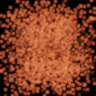
\includegraphics[width=.29\linewidth]{../../../output/profiling/rough-reflections/test-filtered.png} &

\includegraphics[width=.29\linewidth]{../../../output/profiling/rough-reflections/test-reference.png}\\[-1pt]
每个像素取一个方向 & 对左图的倒影降噪 & 每个像素取 512 个方向
\end{tabular}
\end{center}
{\small\color{quiet}Redflag 的 Vulkan 测试。左图的黑底上散着橙色亮点。中图使用同一次取样，单个亮点减少了，仍能看见大小不一的色块。右图用另外 512 个方向取平均，能看清上下两片较亮的倒影与中间稍暗的部分。三张图都用同一亮度显示。\par}

在粗糙度均匀的一小块平面上，相邻像素的位置和朝向相近，能收到的反射光往往也相近。左图已经为每个邻居算了一条反射光线。如果让中心像素借用几份这样的结果，一次恰好采到亮条所造成的误差就有机会减小。但镜面边缘紧挨着墙，或者材料突然从金属变为涂漆时，屏幕上再近的两个点也可能反射完全不同的颜色。

用 $p$ 表示中心像素，$q$ 表示附近的一个像素。记 $R(q)$ 为本次倒影给 $q$ 增添的线性 RGB。让越相近的表面在平均时占越大比重，把这个数叫作权重 $w(p,q)$。把每个 $R(q)$ 乘上它的权重，相加后再除以权重之和。这样即使有几个邻居落在墙面上而被排除，一块颜色均匀的镜面仍能保持原来的亮度。
\[
  \overline R(p)=
  \frac{\sum_{q}w(p,q)\,R(q)}{\sum_{q}w(p,q)} .
\]
举例说，三个像素的红通道是 $1,4,1$，权重分别取 $1,2,1$，得到 $(1+8+1)/4=2.5$。若第三个像素落在镜框上，它的权重改为零，分子与分母都要重新算，结果是 $(1+8)/3=3$。这组数字只为说明平均的算法。

实际计算时还要保住表面原有的照明。把计算倒影前的颜色记为 $B$，加上倒影后的颜色记为 $C$，就有 $R(q)=C(q)-B(q)$。着色器只对这份差值取平均，最后给它加回中心像素自己的 $B(p)$。这样即使相邻像素一个在阴影中、一个被灯直接照亮，它们的直接光仍各自留在原处。

在代码里，\texttt{ScreenEffects::Render} 先让 GPU 把 $C$ 写到一份单独的图里，再把它和原图 $B$ 一起交给降噪着色器。为了检查底图有没有被抹糊，测试把 $B$ 换成隔一个像素就换色的棋盘。用降噪后的图减去棋盘，再与黑底上的倒影逐像素比较，RGB 差值的长度最大仍小于百万分之一。\href{run:../../Redflag/src/Redflag/Renderer/ScreenSpace/ScreenEffects.cpp}{引擎调用}\quad\href{run:../profiling/rough-reflections/test-edges.csv}{棋盘与接缝读数}\quad\href{run:../profiling/rough-reflections/test-capture.json}{RenderDoc 的两次计算}

\clearpage
\subsection{相邻像素的取舍}

GPU 已经保存了相机看到的表面位置 $P$ 和法线 $n$。把两点间的位移 $P_q-P_p$ 沿中心法线 $n_p$ 投影，得到 $d=\lvert (P_q-P_p)\cdot n_p\rvert$。沿一块倾斜的平板移动时，点到相机的距离在变，两点的连线却始终贴着平板，$d$ 仍为零。如果邻点落在墙上，连线会离开平板，$d$ 随之增大。着色器沿邻点的法线也量一次，取两次中较大的距离。

\begin{center}
\begin{tikzpicture}[x=1mm,y=1mm,>=stealth, every node/.style={font=\small,text=ink}]
  \fill[wine!9] (5,3) rectangle (68,6);
  \draw[wine,very thick] (5,6) -- (68,6);
  \fill[ink!9] (87,14) rectangle (151,17);
  \draw[ink,thick] (87,17) -- (151,17);
  \draw[->,quiet] (25,6) -- (25,25) node[above]{中心法线};
  \fill[wine] (25,6) circle (.9) node[below=2mm]{中心 $p$};
  \fill[wine] (56,6) circle (.9) node[above=1mm]{同一平面};
  \draw[quiet,densely dashed] (68,6) -- (129,6);
  \fill[ink] (108,17) circle (.9) node[above=1mm]{另一表面 $q$};
  \draw[<->,wine] (121,6) -- (121,17) node[midway,right]{$d$};
\end{tikzpicture}
\end{center}
{\small\color{quiet}沿中心表面侧看。虚线延长了中心表面所在的平面。图中的 $d$ 是邻点到这个平面的垂直距离，按场景长度计算。\par}

靠近中心的邻居影响更大。横向从左到右的权重取 $1,4,6,4,1$，竖向也取这五个数，相乘便得到每个位置的权重。项目选了最多两圈邻居，粗糙度达到 $0.5$ 时才用满。两点沿法线分开的距离达到半个像素在场景中覆盖的宽度，或法线夹角达到约 $26^\circ$，权重就减到零。两点的底色或金属度差得太多也会分开计算。

\noindent{\small\color{quiet}按计算着色器 \href{run:../../Redflag/src/Redflag/Renderer/ScreenSpace/Shaders/ReflectionFilter.comp}{\texttt{ReflectionFilter.comp}} 整理的伪代码}\par\nopagebreak
\begin{lstlisting}[escapeinside={(*@}{@*)}]
if background(p) or perfectMirror(p): return color[p]
sumRGB = 0
sumWeight = 0
for q in nearbyPixels(p):
    w = sampleWeight(p, q)              (*@{\footnotesize\color{quiet}比较位置、朝向和材质。}@*)
    sumRGB += w * (color[q] - base[q])  (*@{\footnotesize\color{quiet}取邻居的倒影。}@*)
    sumWeight += w
return base[p] + sumRGB / sumWeight
\end{lstlisting}

在 $96\times96$ 的镜面上，把每个像素的红、绿、蓝与参考图对应的数值相减，平方后求平均。再对 16 帧取平均，就得到下表的均方误差。换成与前一帧相减，就能看出镜头固定时颜色还会波动多少。最后一列取亮条与灰条中央的红通道之差。\href{run:../../tests/RoughReflectionCheck.h}{测试代码}\quad\href{run:../profiling/rough-reflections/test-quality.csv}{读数}

\begin{center}\small
\begin{tabular}{@{}lrrr@{}}\toprule
同一镜面 & 对参考图的均方误差 & 相邻帧的均方差 & 灯条红通道差\\\midrule
每像素取一个方向 & \measured{rough-raw-mean_rgb_mse} & \measured{rough-raw-adjacent_rgb_mse} & \measured{rough-raw-bright_minus_middle_red}\\
倒影降噪后 & \measured{rough-filtered-mean_rgb_mse} & \measured{rough-filtered-adjacent_rgb_mse} & \measured{rough-filtered-bright_minus_middle_red}\\
参考图 & --- & --- & \measured{rough-reference-bright_minus_middle_red}\\\bottomrule
\end{tabular}
\end{center}

Dammertz 等人用位置和法线决定哪些样本可以一起平均，并逐轮拉开取样间距。Redflag 只对当前帧平均一次，小于取样范围的细纹仍可能被抹平。AMD 的反射降噪还会估算亮度波动，结合前一帧的颜色继续处理。
\href{https://jo.dreggn.org/home/2010_atrous.pdf}{HPG 2010，图 2、3 与式 (2)--(5)}\quad
\href{https://doi.org/10.2312/EGGH/HPG10/067-075}{论文 DOI}\quad
\href{https://gpuopen.com/manuals/fidelityfx_sdk/techniques/denoiser/}{AMD Denoiser 1.3}\quad
\href{https://github.com/GPUOpen-LibrariesAndSDKs/FidelityFX-SDK/blob/v1.1.4/sdk/include/FidelityFX/gpu/denoiser/ffx_denoiser_reflections_prefilter.h}{AMD 空间滤波源码}\quad
\href{https://pbr-book.org/4ed/Monte_Carlo_Integration/Monte_Carlo_Basics}{PBRT 第四版 §2.1.4，均方误差}


\clearpage
\section{光谱、色散、球谐函数与体素}
\subsection*{从一束光到屏幕颜色}

一面白墙在暖灯下微微发黄。灯发出了什么光，墙又把其中多少光反射到了眼前？把光按波长展开，就得到它的光谱\term{spectrum}。横轴上的波长常用纳米（nm）表示，纵轴告诉我们在各波长附近有多少光。光源可以在许多波长上都有输出，也可以把大部分能量集中在很窄的一段。同样明亮的两盏灯，光谱的形状也可能很不一样。

先只比较两个同样宽的窄波段。假设蓝光附近和红光附近各有 4 份光落在一块颜料上。颜料在蓝光附近反射四分之一，在红光附近反射四分之三。于是反射出去的蓝光有 1 份，红光有 3 份。这个算法可以对每一小段波长分别做一次。用 $\lambda$ 表示波长，$S_{\rm in}$ 表示落在表面的光谱，$\rho$ 表示该波长的反射比例。对普通的漫反射颜料，把各波长相同的几何因素暂时略去，有
\[
  S_{\rm out}(\lambda)=S_{\rm in}(\lambda)\,\rho(\lambda).
\]
\begin{center}
\small
\begin{tabular}{@{}lrrr@{}}
\toprule
比较的窄波段 & 落在颜料上的光 & 反射比例 & 反射出去的光 \\
\midrule
450 nm 附近（蓝）& 4 份 & $1/4$ & 1 份\\
650 nm 附近（红）& 4 份 & $3/4$ & 3 份\\
\bottomrule
\end{tabular}
\end{center}

显示器需要的是红、绿、蓝三个数。可以先用三条颜色匹配曲线对光谱分别做加权求和，得到标准颜色空间 CIE XYZ 中的三个数，再换算成显示用的 RGB。例如 $Y$ 对应人眼在明亮环境下的亮度响应，$\bar y(\lambda)$ 是不同波长的权重，$k$ 取决于使用的单位。下面的积分就是把每一小段波长的贡献相加。
\[
  Y=k\int_{\text{可见光}} S_{\rm out}(\lambda)\,\bar y(\lambda)\,{\rm d}\lambda .
\]
三次求和会丢失细节。两块色样在一盏灯下可以看成同色，换一盏光谱不同的灯，各波长参加求和的比重变了，色样就可能显出差别。

再回到编辑器里的那面墙。底色贴图已经把颜色存成 RGB，GI 着色器把读到的 sRGB 转为线性值，便可将底色与灯光逐分量相乘。假设灯光是 $(1,0.5,0.25)$，墙面刷上 $(0.8,0.4,0.2)$ 的漆，乘完得到 $(0.8,0.2,0.05)$，之后还要考虑入射角和距离。把墙重新刷白，三个分量就能保留更多灯光原有的颜色。若想预测两块同色的漆换灯之后能否分辨出来，仅有这三个数已经不够，还需要颜料和灯光的光谱。

\noindent{\small\color{quiet} 对照阅读\enspace
\href{https://pbr-book.org/4ed/Radiometry,_Spectra,_and_Color/Representing_Spectral_Distributions}{PBRT 第四版 §4.5，图 4.16 柠檬皮的反射曲线}；
\href{https://pbr-book.org/4ed/Radiometry,_Spectra,_and_Color/Color}{§4.6，图 4.18 颜色匹配曲线}。
项目入口是 \href{run:../../Redflag/src/Redflag/Renderer/GI/Shaders/GI.comp}{GI.comp} 的 \texttt{linearTexel} 和 \texttt{direct}。}

\clearpage
\subsection*{棱镜中的色散}

把一束窄的白光射入玻璃棱镜，另一侧能看到颜色逐渐展开。白光本来就包含许多波长。普通玻璃对不同波长有略微不同的折射率 $n(\lambda)$，光从空气斜着进入玻璃时，各波长在界面处转过的角度便有细小差别。这种光学性质称为色散\term{dispersion}。

\begin{center}
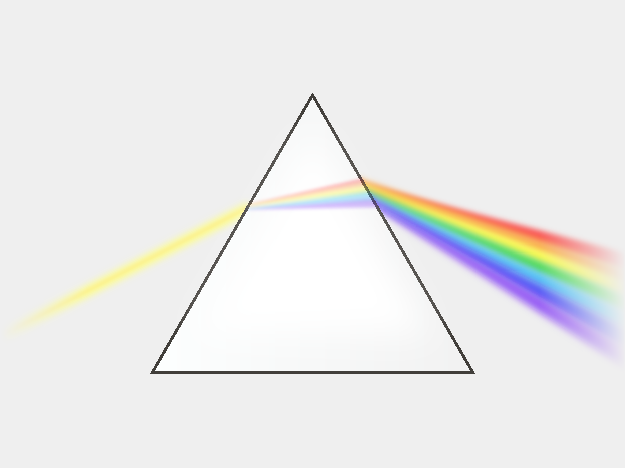
\includegraphics[width=.48\linewidth]{figures/prism-rainbow.pdf}\\[-1pt]
{\small 从入射光束沿玻璃向右看，出射一侧可以分辨不同波长的方向。}\\
{\footnotesize\color{quiet}\href{https://commons.wikimedia.org/wiki/File:Prism-rainbow.svg}{Suidroot，\emph{Prism-rainbow}，2008}，
\href{https://creativecommons.org/licenses/by-sa/4.0/}{CC BY-SA 4.0}。原图转为 PDF。}
\end{center}

角度要从界面的法线量起。法线就是穿过入射点、垂直于玻璃表面的直线。设入射角为 $\theta_i$，进入玻璃后的角为 $\theta_t$，斯涅尔定律写作
\[
  n_{\text{空气}}\sin\theta_i=n_{\text{玻璃}}(\lambda)\sin\theta_t(\lambda).
\]
取空气折射率为 1，让入射角等于 $30^\circ$，左边就是 $1/2$。为了看清差别，把红光和蓝光的折射率分别取为 $1.50$ 和 $1.60$，这组教学数值放大了色散。红光在玻璃里的角度满足 $\sin\theta_t=1/3$，约为 $19.5^\circ$。蓝光得到 $5/16$，约为 $18.2^\circ$，在这里更靠近法线。棱镜的第二个面与第一个面不平行，出射后两束光沿不同方向前进，在远处的屏上就能分开。

设想用渲染器把这束光一直追到白屏上。红光射到屏幕的哪个点，要用红光的折射率穿过两道玻璃表面才能知道，蓝光则要用它自己的折射率再算一遍。等各波长到达各自的像素，才合成为屏幕颜色。前面照亮墙面的 RGB 漫反射在同一条光路上计算三个分量。当前引擎还没有沿不同波长分别追踪玻璃折射的步骤。

\noindent{\small\color{quiet} 同一玻璃场景的两次渲染见
\href{https://pbr-book.org/4ed/Reflection_Models/Specular_Reflection_and_Transmission}{PBRT 第四版 §9.3.1，图 9.9}。比较玻璃投下的亮斑，可以看到固定折射率和随波长变化的折射率给出的差别。}

\clearpage
\subsection*{窗边的石膏球}

把一个灰色石膏球搬到窗边。朝向天空的一面较亮，朝向地面的一面较暗。给球着色时，光是知道球心在窗边还不够，还要知道每一小块球面朝向哪里。第~\ref{lesson-ddgi}~章的探针在窗旁取样时，以世界坐标的六个正负轴为中心，分别向对应半球发射光线，留下六组 RGB 平均值和命中距离统计。

给石膏球的顶端着色，程序只取 $+y$ 那一组。走到斜面，法线 $n$ 恰好在 $+x$ 与 $+y$ 之间，每组按 $\max(0,n\cdot a)^2$ 参与，其中 $a$ 是这一组的轴向。这两组各占 $(1/\sqrt2)^2=1/2$。石膏球放在几个探针之间时，还要结合距离和遮挡混合附近八个探针。整个计算直接读取各方向的值。

也可以把天空的明暗看成一幅铺在单位球面上的图。用 $\omega$ 表示从球心指向球面的单位方向，以 $+y$ 为上，假设一个颜色分量的亮度是 $L(\omega)=2+\omega_y$。这个图样可以分两笔画成。先把整个球涂成亮度 2，再叠加一层从下往上逐渐变亮的图样。在下方，第二笔让原来的亮度减去 1。

\begin{center}
\begin{tikzpicture}[x=.77cm,y=.67cm,font=\small]
  \draw[quiet!35] (0,0) circle[x radius=1.38,y radius=1.38];
  \foreach \a/\b in {0/1.26,1.26/0,0/-1.26} \draw[->,thick,wine] (0,0)--(\a,\b);
  \fill[ink] (0,0) circle (2pt);
  \node[anchor=east] at (-1.55,0) {探针};
  \draw[quiet] (-1.42,0)--(-.16,0);
  \node[anchor=west] at (.44,1.17) {向上\quad $2+1=3$};
  \node[anchor=west] at (1.62,0) {水平\quad $2+0=2$};
  \node[anchor=west] at (.44,-1.17) {向下\quad $2-1=1$};
\end{tikzpicture}\\
{\small 本册绘制。在同一个探针位置，向三个方向读取例子里的亮度。}
\end{center}

球谐函数\term{spherical harmonics, SH}给出了一套可以这样叠加的球面函数。最低一层处处相同，下一层描述三个方向上的渐变，再下一层还能表示更细的起伏。用 $Y_{\ell m}$ 记第 $\ell$ 层中的一个函数，$c_{\ell m}$ 记它在当前光照里占多少。选取正交归一的实球谐基时，前三层的近似为
\[
 c_{\ell m}=\int_{S^2}L(\omega)Y_{\ell m}(\omega)\,{\rm d}\omega ,
 \qquad
 L(\omega)\approx\sum_{\ell=0}^{2}\ \sum_{m=-\ell}^{\ell} c_{\ell m}Y_{\ell m}(\omega).
\]
左边沿整个球面求和，计算光照与每一种分布的吻合程度。右边在所问方向上把它们加回来。三层各有 $1,3,5$ 个函数，每个颜色分量需要 9 个系数。前面例子里的 $2$ 和 $1$ 是常数和方向余弦的倍率，换成归一化的球谐基时倍率会相应换算。漫反射表面汇集来自一大片方向的光，把细小的亮暗变化抹平，因而适合这种低阶近似。若要保留镜面里一颗很小的太阳，九个数就太少了。换成一颗金属球，粗糙度还会改变倒影的清晰程度。配套的\href{run:Redflag-Rendering-Math.pdf}{《渲染公式与实现》}用 OpenGL 的环境贴图来画这种表面。

\noindent{\small\color{quiet} \href{https://graphics.stanford.edu/papers/envmap/}{Ramamoorthi 与 Hanrahan，漫反射环境光的球谐近似（2001）}；
\href{https://sites.cs.ucsb.edu/~lingqi/teaching/resources/GAMES202_Lecture_06.pdf}{闫令琪，GAMES202 第六讲球谐基图示}。
\href{run:../../Redflag/src/Redflag/Renderer/GI/Shaders/GI.comp}{项目实现}见 \texttt{updateProbe} 和 \texttt{gatherProbes}。}

\clearpage
\subsection*{墙面与体素}

一束光穿过房间，最后碰到墙。前面的间接光算法要找准确的撞击点，于是用包围盒树（BVH）先跳过整组碰不到的三角形，再对剩下的三角形求交。换个问题，若只关心“房间的哪一小块空间被墙占着”，可以预先把空间切成等大的小立方体，在与墙面相交的格子里留下标记。这样的三维格子叫作体素\term{voxel}，把三角形模型写入这些格子的过程就叫体素化。

设格网原点为 $(0,0,0)$，每格边长 $h=0.5$ 米。要找墙上一点 $p=(1.2,0.3,0.8)$ 米落在哪一格，先用各坐标除以边长，再分别向下取整。这样得到从 0 开始数的格号。
\[
 (i_x,i_y,i_z)=\lfloor p/h\rfloor
   =\lfloor(2.4,0.6,1.6)\rfloor=(2,0,1).
\]
\begin{center}
\begin{tikzpicture}[x=.78cm,y=.78cm,font=\small]
  \fill[wine!17] (2,1) rectangle (3,2);
  \draw[step=1,gray!65] (0,0) grid (4,3);
  \draw[->,thick] (0,0)--(4.38,0) node[right] {$x$};
  \draw[->,thick] (0,0)--(0,3.36) node[above] {$z$};
  \foreach \x in {0,1,2,3} \node[below] at (\x+.5,0) {\x};
  \foreach \z in {0,1,2} \node[left] at (0,\z+.5) {\z};
  \fill[wine] (2.4,1.6) circle (3pt);
  \draw[wine] (2.4,1.6)--(4.8,2.05)--(5.2,2.05);
  \node[anchor=west] at (5.2,2.05) {墙上的点 $p$};
  \node[anchor=west,text=quiet] at (5.2,1.2) {淡红色表示它落入的格子};
\end{tikzpicture}\\
{\small 本册绘制。从上方看第 $i_y=0$ 层。坐标轴下方和左边标出格号，每格宽半米。}
\end{center}

若按 $x$ 最快、其次 $y$、最后 $z$ 的顺序存储，设每行有 4 个格子，每层有 3 行，格号 $(2,0,1)$ 的数组下标就是 $2+4(0+3\times1)=14$。格子越小，斜墙的轮廓越贴近原来的三角形。若把三个方向都细分一倍，并给每个格子分配存储，格数就增为 $2^3=8$ 倍。稀疏结构只为需要记录的区域分配空间，可以减轻这项开销。

现在在窗前添一小团烟。若每格记录烟的密度，就可以沿光路一格一格地读。假设前三格一样厚，光在各格穿出后分别剩下进入时的全部、一半和一半。那么 4 份光穿过第一格仍有 4 份，穿过第二格剩 2 份，穿过第三格就只剩 1 份。这里每一格都代表房间里的固定位置，转动相机后烟仍在原处。第~\ref{lesson-cluster}~章给点光源分簇时也能看到格子，但那些格子随相机移动，存的是哪些灯可能照到画面的这一块。当前引擎靠三角形求墙面交点，例子里的密度格网则是画烟时可以另选的一种表示。

\noindent{\small\color{quiet} \href{https://michael-schwarz.com/research/publ/2010/vox/}{Schwarz 与 Seidel，三角网格的体素化（2010）}；
\href{https://pbr-book.org/4ed/Volume_Scattering/Media}{PBRT 第四版 §11.4，格网介质}；
\href{run:../../Redflag/src/Redflag/Renderer/GI/GIScene.cpp}{项目包围盒树}；
\href{run:../../Redflag/src/Redflag/Renderer/ScreenSpace/Shaders/Cluster.glsl}{屏幕分簇的下标与深度}。}

\clearpage
\section{雾中的点光源}
Sponza 的三盏点光源悬在走廊上方。左图里，读者主要从柱面和挂毯的亮度判断灯在何处。右图里，连灯前面的空气也亮了起来。两个画面用同一组灯和相机。打开 Vulkan 编辑器，在「实时效果」里勾选「体积雾」，就可以在组合光照 Lit 里看见这个变化。

\begin{center}
\begin{minipage}{.485\linewidth}\centering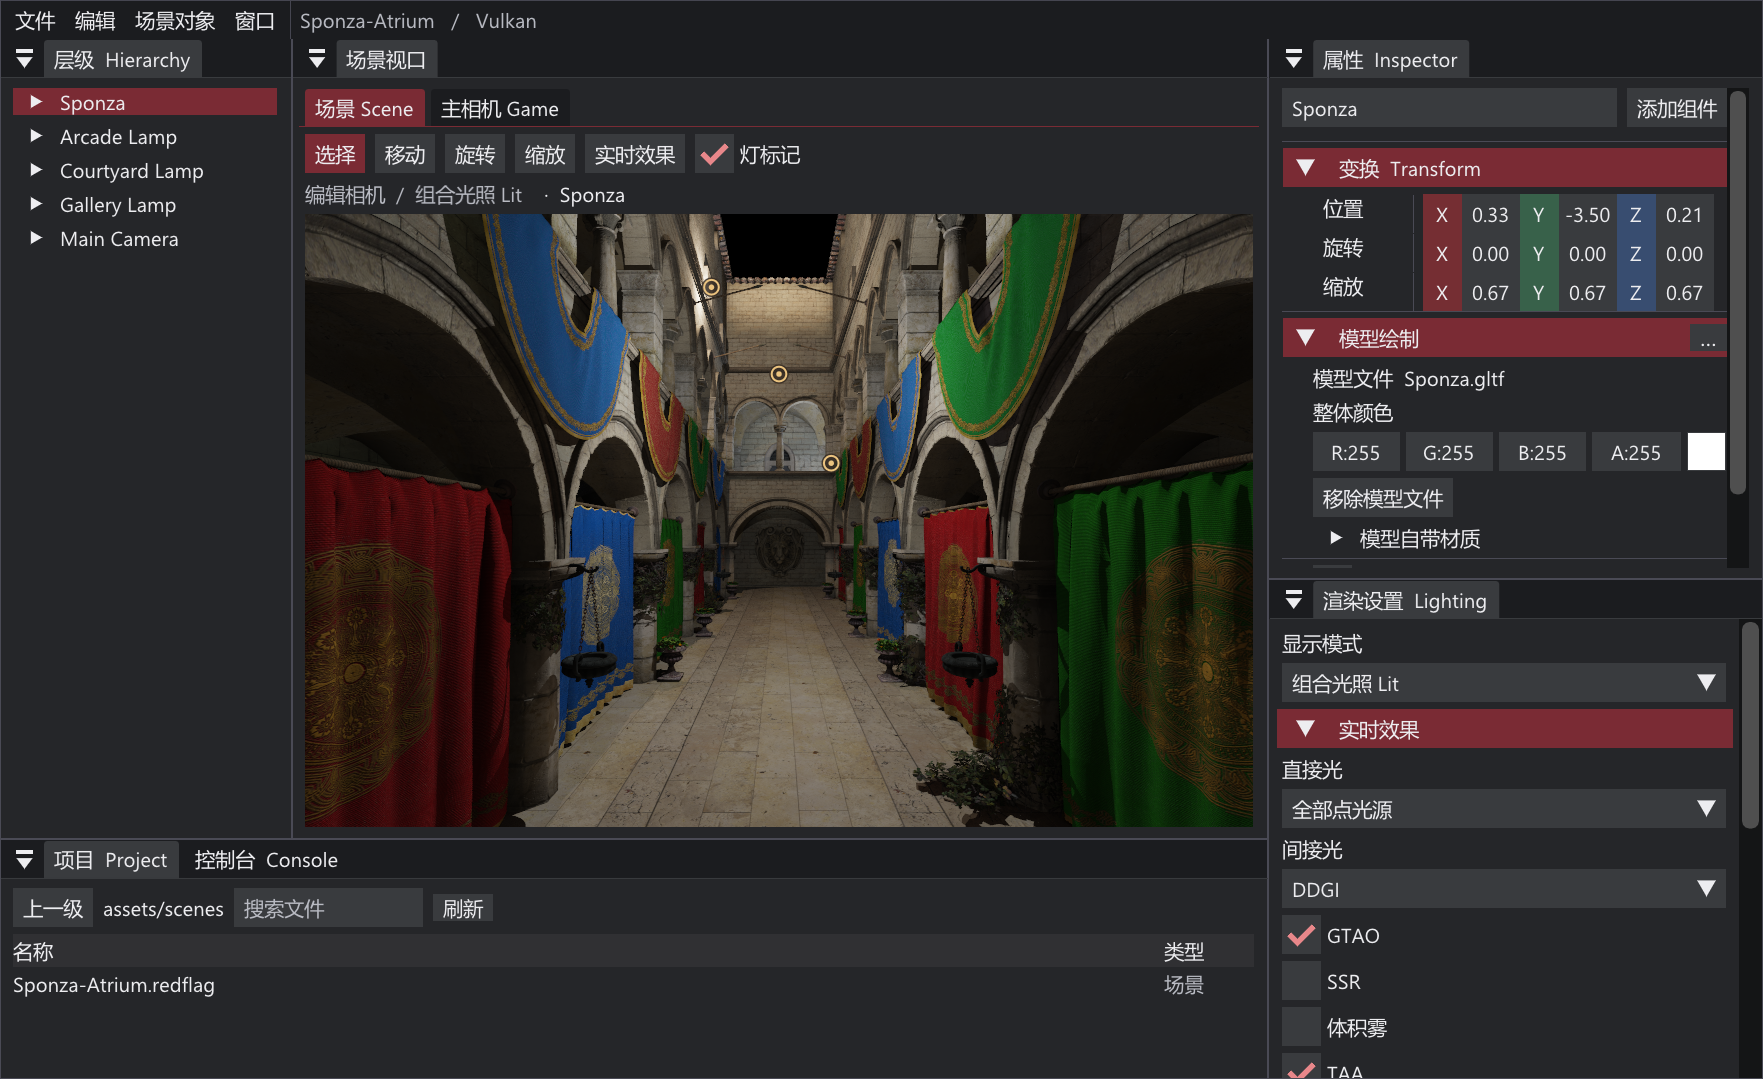
\includegraphics[width=\linewidth,trim=305bp 252bp 510bp 214bp,clip]{../../../output/profiling/fog/sponza-clear.png}\\{\small 体积雾关闭}\end{minipage}\hfill
\begin{minipage}{.485\linewidth}\centering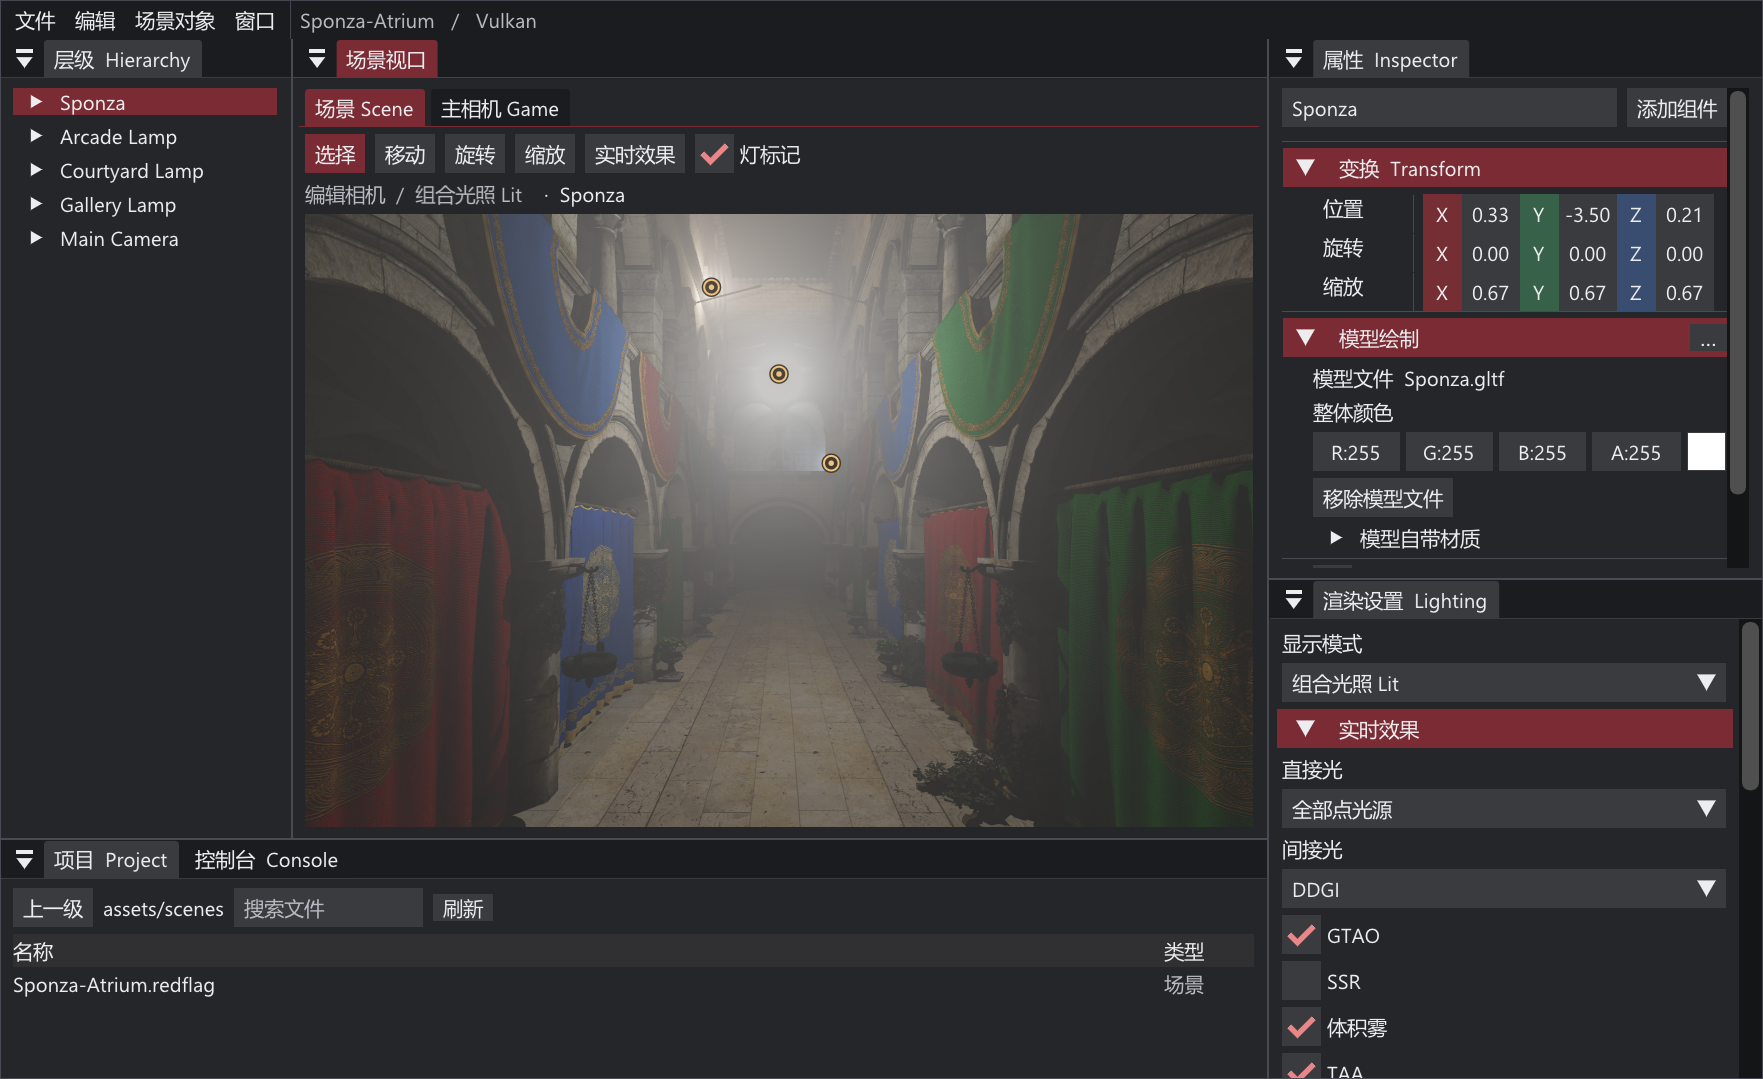
\includegraphics[width=\linewidth,trim=305bp 252bp 510bp 214bp,clip]{../../../output/profiling/fog/sponza-fog.png}\\{\small 体积雾开启}\end{minipage}
\end{center}
{\small\color{quiet}Redflag 正式 Vulkan 编辑器，$948\times613$。雾密度 0.10，散射比例 0.92，散射方向 0.35，最远距离 24，16 步。}

先看远端的拱门。表面反射的光要穿过空气才到达镜头。假设穿过一个世界单位后还剩原来的 90.5\%，穿过两段就剩 $0.905^2$。把雾密度记作 $\sigma_t$，距离记作 $d$，穿过整段后能保留的比例为 $T(d)=\exp(-\sigma_t d)$。取右图的 $\sigma_t=0.10$，一段长 10 的路只剩 $e^{-1}\approx0.368$。面板中的「雾密度」使用每世界单位的消光系数，场景若按米建模，单位就是每米。

再看灯附近的白雾。有些光离开点光源，还没碰到地面便被雾滴散射，其中一部分转向镜头。程序沿一个像素的视线取样。若采样点与灯之间隔着墙，该灯就照不到这里。穿过窗洞的光只照亮那些能看见灯的采样点，于是雾里出现一束带轮廓的光。

\begin{center}
\begin{tikzpicture}[font=\small,>=stealth]
\draw[fill=shade,draw=quiet!40,rounded corners] (0,0) rectangle (13.4,2.55);
\node at (1.0,.44){镜头};\node at (11.9,.44){可见表面};
\draw[->,very thick,wine] (1,.85)--(11.8,.85);
\foreach \x in {2.4,4.4,6.4,8.4,10.4}{\fill[wine] (\x,.85) circle (2.4pt);}
\node at (5.5,2.18){点光源};\draw[->,quiet] (5.5,1.97)--(4.45,.94);
\draw[dashed,quiet] (5.8,1.98)--(8.35,.9);
\draw[line width=2pt] (7.2,1.05)--(7.2,1.8);
\node[fill=shade,inner sep=1pt] at (9.25,1.86){墙挡住了右侧的光};
\end{tikzpicture}
\end{center}
{\small\color{quiet}本册绘制。红点是每一小段的中点。视线在最近的表面结束，穿墙之后的雾不会叠在墙前。}

\clearpage
\subsection*{沿视线积累光照}
把长度 $d$ 切成 $N$ 段，每段长 $h=d/N$。设 $a$ 为单次散射比例，$L_s$ 为中点处从各盏灯到达、并按散射方向加权后的入射亮度。单段中，直线传过的比例是 $t=e^{-\sigma_t h}$，离开原来方向的比例就是 $1-t$。把入射亮度近似看成这一小段内恒定，散射到镜头方向的增量是 $a(1-t)L_s$。它还要穿过镜头与该段之间的雾。第 $j$ 段从零计数，最后的像素为
\[
 L_{\rm pixel}=t^N L_{\rm surface}
   +\sum_{j=0}^{N-1}t^j\, a(1-t)\,L_{s,j}.
\]
\noindent{\small\color{quiet}按 GLSL 整理的伪代码\quad\href{run:../../Redflag/src/Redflag/Renderer/GI/Shaders/Fog.comp}{\texttt{Fog.comp}}}\par\nopagebreak
\begin{lstlisting}[escapeinside={(*@}{@*)}]
T = 1; scattered = 0
for each segment from the camera:
    point = midpoint(segment)
    incident = sum_visible_point_lights(point, viewRay)
    (*@{\footnotesize\color{quiet}这一段散向镜头的光，还要穿过前面各段雾。}@*)
    scattered += T * albedo * (1 - stepT) * incident
    T *= stepT
output = scattered + T * surfaceColor
\end{lstlisting}

例如一层雾让 80\% 的表面光穿过，散射比例为 0.75。设这层雾从可见灯光得到的方向加权亮度为 2，朝镜头散射的增量就是 $0.75\times0.2\times2=0.3$。若它的前面还有一层同样的雾，到达镜头的这份增量会降到 $0.8\times0.3=0.24$。程序中的 \texttt{T} 便是沿途这些比例的乘积。

\pair{profiling/fog/open.png}{点光源穿过方孔}{profiling/fog/closed.png}{同一盏灯，方孔封住}
{\small\color{quiet}同一个 Vulkan 离屏场景，$384\times216$，32 步。右半部中央的取样位置在左上角起算的 $(288,108)$；封住小孔后，这里的线性红色分量从 0.02275 降为 0。}

\clearpage
\subsection*{编辑器中的取值与检查}
雾较稀时，可以先把「雾密度」设为 0.03，把「散射方向」设为 0，这样从各个方向观察同一团雾都使用相同的散射权重。想让逆光更明显，可逐步调高散射方向。它控制 Henyey--Greenstein 相函数中的 $g$，也就是入射方向与散射后方向之间的平均余弦。正值偏向继续向前传播的光，负值偏向散回光源一侧。着色器使用
\[
p_g(c)=\frac{1-g^2}{4\pi(1+g^2-2gc)^{3/2}},
\qquad c=\hat{\boldsymbol l}\cdot\hat{\boldsymbol v}.
\]
单位向量 $\hat{\boldsymbol l}$ 从采样点指向灯，$\hat{\boldsymbol v}$ 从镜头指向采样点。它们都和光实际旅行的方向相反，一起取反不改变点积。灯到采样点这段还要乘 $e^{-\sigma_t r}$ 和距离平方的倒数，$r$ 是到灯的距离。每盏灯沿用点光源属性中的半径，雾与表面在同一半径外都收不到这盏灯的光。实现将平方距离的最小值取为 $0.04$，相当于在距点光源 0.2 个单位以内限制亮度，避免单个采样点恰落在灯心时失控。

\begin{fields}
\texttt{FogSettings} & 保存密度、散射比例、散射方向、最远距离和步数。体积雾默认关闭，打开后这些值跟随场景的 \texttt{.render.yaml} 保存。\\
\texttt{RenderFog} & 接收线性场景颜色。每个像素用 \texttt{GISurface} 找到最近表面；背景沿视线算到最远距离或相机远平面。\\
\texttt{Fog.comp} & 中点到每盏点光源的遮挡使用场景三角形的层次包围盒。结果先交给 TAA，再由显示着色器调亮度。\\
\end{fields}

图中方孔测试用了恒定密度的雾。关灯、将表面输入设为白色后，画面应只剩透过来的白光。测试按各像素自己到表面的距离计算理论值，82,944 个像素中最大的绝对误差为 $3.13\times10^{-7}$。打开灯再封住方孔，照不到的区域应重新变暗。另将半径从无限缩为一个单位。镜头中央的视线距离灯约三单位，红通道从 0.299884 降到 0.244632，与关灯时相等。

缩短「雾的最远距离」会截去远处的雾。增大步数会减轻窄光束上的条带，也会增加遮挡查询。在方孔小场景中，32 步的单次计算在 RenderDoc 回放中用时约 0.41 毫秒；完整 Sponza 有更多三角形和点光源，要另行测量。这一版采用均匀介质的单次散射，表面照明仍来自已有的 Lit 计算。较浓的雾里，散射多次才到达眼睛的光还没有计入。

{\small\color{quiet}\href{https://pbr-book.org/4ed/Volume_Scattering/Transmittance}{PBRT 第四版，§11.2 Transmittance}；
\href{https://pbr-book.org/4ed/Volume_Scattering/Phase_Functions}{§11.3 Phase Functions}；
\href{https://github.com/mmp/pbrt-v4}{PBRT v4 作者源码}；
\href{https://www.realtimerendering.com/advances/s2015/index.html}{S. Hillaire，SIGGRAPH 2015 课程，Physically-based and Unified Volumetric Rendering in Frostbite}。Frostbite 课程采用分块的体积网格，本项目沿各像素的视线积分。测试入口为 \texttt{tests/run\_fog\_tests.cmd}。}

\clearpage
\section{镜头外的灯牌照亮白墙}

把一盏灯牌架在白墙前面，让发光的一侧朝墙。相机也朝墙，但画面只取灯牌左侧的一小块。把场景里的点光源全部关掉，这块白墙原本会变成黑色。要让它亮起来，从墙面出发的光线就得找到镜头外的灯牌，并带回打中那个位置的颜色。

沿墙面法线朝向的半球取一条射线，找到它打中的第一块三角形。如果这块表面会发光，就按交点的 UV 找到纹素，先从 sRGB 转为线性 RGB，再乘材质中的发光颜色与强度。单面灯牌只有正面发光；双面灯牌的背面也可以照亮墙。\href{https://registry.khronos.org/glTF/specs/2.0/glTF-2.0.html#material-emissivetexture}{glTF 2.0，发光贴图}

\begin{center}
\begin{tabular}{@{}cccc@{}}

\includegraphics[width=.20\linewidth]{../../../output/profiling/emissive-gi/reference.png}&

\includegraphics[width=.20\linewidth]{../../../output/profiling/emissive-gi/live-three.png}&

\includegraphics[width=.20\linewidth]{../../../output/profiling/emissive-gi/live-sixteen.png}&

\includegraphics[width=.20\linewidth]{../../../output/profiling/emissive-gi/baked.png}\\
面积积分 & 每方向 3 条 & 每方向 16 条 & 烘焙后
\end{tabular}
\end{center}
{\small 左图按灯牌的位置与两个纹素独立算出。后三图是 Vulkan 输出的同一小块墙，原始大小均为 $17\times17$。中间两图取第 24 帧。四张图都用 $1-e^{-2L}$ 调亮并转成 sRGB，下面的数值直接读原始线性颜色。\par}

这块测试灯牌宽 1.2、高 1，与墙平行，两者相隔一个场景单位。把灯牌分成 $128\times96$ 个小方块。站在墙上一点 $x$ 看某个小块 $y$，离得远，它占的视角就小；斜着看，它看起来也会窄。设两点距离是 $r$，连线与两侧法线的夹角分别是 $\theta_x,\theta_y$，小块面积为 $\Delta A$。让每个小块发出的颜色 $L_e(y)$ 乘上这些比例，再乘白墙的漫反射率 $\rho=0.8$，把各块的贡献加起来，就有了参考值。
\[
  L_o(x)\;\approx\;\frac{\rho}{\pi}\sum_y L_e(y)
    \frac{\cos\theta_x\cos\theta_y}{r^2}\,\Delta A .
\]
灯牌的左纹素是纯红色 255，右纹素的绿色是 128。绿色解码后约为 0.216，乘绿色因子 0.5 和强度 4，约为 0.432。这两个数指灯牌自身发出的颜色。传到墙面还要经过上式，整块墙的参考平均值降到了 $(0.215215,0.014061,0)$。GPU 从每个墙面像素发出 2,048 条射线，得到 $(0.215356,0.014110,0)$。ReSTIR GI 每像素每帧只有一个新候选，512 帧平均是 $(0.213964,0.014929,0)$。\href{https://pbr-book.org/4ed/Light_Sources/Area_Lights}{PBRT 第四版 §12.4}

DDGI 会先让附近的探针观察灯牌，再用这些探针估计墙上的光。每个方向从 3 条射线增到 16 条后，上图的深浅变化平缓了一些。把相邻像素的红色差与面积积分作比较，误差从 0.01024 降到 0.00475；但整幅画的红色平均值也从 0.21282 变为 0.17053。增加射线能减轻起伏，探针之间插值造成的偏差仍在。烘焙后这块墙的平均红色为 0.19981。关掉应用再打开，289 个像素的四个浮点分量与之前完全相同。要继续改善大墙上的色斑，可以先让窄灯牌占据的方向更容易被取到，再用同一机位检查相邻像素和平均颜色两个指标。

\href{run:../../tests/EmissiveGICheck.h}{面积积分与 Vulkan 回归}\quad\href{run:../profiling/emissive-gi/measurements.csv}{逐项读数}

\clearpage
\section{光线与场景中的三角形}
雾里的一点能否被灯照亮，取决于它和灯之间有没有墙。场景里有几十万个三角形，逐个检查会很慢。加载模型时，CPU 给一组相邻的三角形套上长方体，称为包围盒；再把这组分小，直到一个盒子里最多剩下六个三角形。这样组成的树叫作包围盒层次结构（BVH）。GPU 查遮挡时，先试光线能否穿过大盒子。连盒子都碰不到，里面的三角形就可以一起跳过。

\begin{center}
\begin{tikzpicture}[x=.92cm,y=.62cm,font=\small]
\foreach \y/\labeltext in {2.4/各取八个,0/沿空隙分开}{
  \node[anchor=east] at (-.35,\y+.5) {\labeltext};
  \foreach \x in {0,1,2,9}{
    \fill[quiet!15] (\x,\y+.07) rectangle ++(1,.86);
    \draw[quiet!60] (\x,\y+.07) rectangle ++(1,.86);
    \draw[quiet!60] (\x,\y+.07) -- ++(1,.86) (\x,\y+.93) -- ++(1,-.86);
  }
}
\draw[wine,thick,rounded corners=1pt] (-.04,2.32) rectangle (1.97,3.48);
\draw[teal!70!black,thick,rounded corners=1pt] (2.02,2.32) rectangle (10.04,3.48);
\draw[wine,thick,rounded corners=1pt] (-.04,-.08) rectangle (3.04,1.08);
\draw[teal!70!black,thick,rounded corners=1pt] (8.96,-.08) rectangle (10.04,1.08);
\foreach \y in {0,2.4}{\draw[->,thick] (5.5,\y+1.6) -- (5.5,\y+.35);}
\end{tikzpicture}
\end{center}
{\small\color{quiet}俯视示意，按本项目的划分方法绘制。每个灰格代表四个三角形，彩框是分出来的两个盒子。箭头穿过同一条空走廊。上图还要进入右边的盒子查找，下图在两个盒外就能排除遮挡。}\par

怎样估算一种划分要做多少工作？从许多方向发出射线时，较大的盒子通常更容易被穿过。设左右盒子的表面积为 $S_L,S_R$，其中的三角形数为 $N_L,N_R$，便可用 $S_LN_L+S_RN_R$ 比较同一个父盒里的划分。图中每个灰格的长、宽、高都是 1。上图的盒长分别为 2 和 8，表面积分别为 10 和 34，得分为 $10\times8+34\times8=352$。下图的盒长为 3 和 1，得分降为 $14\times12+6\times4=192$。两图总共有同样多的三角形，差别来自盒子包进了多少空地。

在 \texttt{GIScene.cpp} 的 \texttt{SplitTriangles} 中，CPU 沿三角形中心分布最宽的方向分成 12 段，比较中间的 11 个分界。每比较一次只需要两侧的盒子与个数。代码用半个表面积乘个数，所有得分同时除以二，选出来的位置相同。三角形很少或中心重合时，直接平分。画面渲染期间，GPU 沿建好的树查找。查阴影只要在灯前遇到一块不透明表面就能停，查反射则要保留最近交点，才能读到正确的材质。

{\small\color{quiet}\href{https://pbr-book.org/4ed/Primitives_and_Intersection_Acceleration/Bounding_Volume_Hierarchies}{PBRT 第四版 §7.3.2，按表面积划分包围盒}
\quad\href{run:Redflag-Debugging-Notes.pdf}{墙面接缝的排错图}
\quad\href{run:Redflag-Rendering-Performance.pdf}{两座建筑的 GPU 实测}}\par

\end{document}
